\documentclass[twoside]{book}

% Packages required by doxygen
\usepackage{calc}
\usepackage{doxygen}
\usepackage{graphicx}
\usepackage[utf8]{inputenc}
\usepackage{makeidx}
\usepackage{multicol}
\usepackage{multirow}
\usepackage{textcomp}
\usepackage[table]{xcolor}

% Font selection
\usepackage[T1]{fontenc}
\usepackage{mathptmx}
\usepackage[scaled=.90]{helvet}
\usepackage{courier}
\usepackage{amssymb}
\usepackage{sectsty}
\renewcommand{\familydefault}{\sfdefault}
\allsectionsfont{%
  \fontseries{bc}\selectfont%
  \color{darkgray}%
}
\renewcommand{\DoxyLabelFont}{%
  \fontseries{bc}\selectfont%
  \color{darkgray}%
}

% Page & text layout
\usepackage{geometry}
\geometry{%
  a4paper,%
  top=2.5cm,%
  bottom=2.5cm,%
  left=2.5cm,%
  right=2.5cm%
}
\tolerance=750
\hfuzz=15pt
\hbadness=750
\setlength{\emergencystretch}{15pt}
\setlength{\parindent}{0cm}
\setlength{\parskip}{0.2cm}
\makeatletter
\renewcommand{\paragraph}{%
  \@startsection{paragraph}{4}{0ex}{-1.0ex}{1.0ex}{%
    \normalfont\normalsize\bfseries\SS@parafont%
  }%
}
\renewcommand{\subparagraph}{%
  \@startsection{subparagraph}{5}{0ex}{-1.0ex}{1.0ex}{%
    \normalfont\normalsize\bfseries\SS@subparafont%
  }%
}
\makeatother

% Headers & footers
\usepackage{fancyhdr}
\pagestyle{fancyplain}
\fancyhead[LE]{\fancyplain{}{\bfseries\thepage}}
\fancyhead[CE]{\fancyplain{}{}}
\fancyhead[RE]{\fancyplain{}{\bfseries\leftmark}}
\fancyhead[LO]{\fancyplain{}{\bfseries\rightmark}}
\fancyhead[CO]{\fancyplain{}{}}
\fancyhead[RO]{\fancyplain{}{\bfseries\thepage}}
\fancyfoot[LE]{\fancyplain{}{}}
\fancyfoot[CE]{\fancyplain{}{}}
\fancyfoot[RE]{\fancyplain{}{\bfseries\scriptsize Generated on Fri May 31 2019 14\-:03\-:56 for Tool\-D\-A\-Q\-Framework by Doxygen }}
\fancyfoot[LO]{\fancyplain{}{\bfseries\scriptsize Generated on Fri May 31 2019 14\-:03\-:56 for Tool\-D\-A\-Q\-Framework by Doxygen }}
\fancyfoot[CO]{\fancyplain{}{}}
\fancyfoot[RO]{\fancyplain{}{}}
\renewcommand{\footrulewidth}{0.4pt}
\renewcommand{\chaptermark}[1]{%
  \markboth{#1}{}%
}
\renewcommand{\sectionmark}[1]{%
  \markright{\thesection\ #1}%
}

% Indices & bibliography
\usepackage{natbib}
\usepackage[titles]{tocloft}
\setcounter{tocdepth}{3}
\setcounter{secnumdepth}{5}
\makeindex

% Hyperlinks (required, but should be loaded last)
\usepackage{ifpdf}
\ifpdf
  \usepackage[pdftex,pagebackref=true]{hyperref}
\else
  \usepackage[ps2pdf,pagebackref=true]{hyperref}
\fi
\hypersetup{%
  colorlinks=true,%
  linkcolor=blue,%
  citecolor=blue,%
  unicode%
}

% Custom commands
\newcommand{\clearemptydoublepage}{%
  \newpage{\pagestyle{empty}\cleardoublepage}%
}


%===== C O N T E N T S =====

\begin{document}

% Titlepage & ToC
\hypersetup{pageanchor=false}
\pagenumbering{roman}
\begin{titlepage}
\vspace*{7cm}
\begin{center}%
{\Large Tool\-D\-A\-Q\-Framework }\\
\vspace*{1cm}
{\large Generated by Doxygen 1.8.5}\\
\vspace*{0.5cm}
{\small Fri May 31 2019 14:03:56}\\
\end{center}
\end{titlepage}
\clearemptydoublepage
\tableofcontents
\clearemptydoublepage
\pagenumbering{arabic}
\hypersetup{pageanchor=true}

%--- Begin generated contents ---
\chapter{Configure files}
\label{md_configfiles_README}
\hypertarget{md_configfiles_README}{}
\DoxyHorRuler{0}
 \#\+Description \DoxyHorRuler{0}


Configure files are simple text files for passing variables to the Tools.

Text files are read by the \mbox{\hyperlink{classStore}{Store}} class (src/\+Store) and automatically asigned to an internal map for the relavent \mbox{\hyperlink{classTool}{Tool}} to use.

\DoxyHorRuler{0}
 \#\+Useage \DoxyHorRuler{0}


Any line starting with a \char`\"{}\#\char`\"{} will be ignored by the \mbox{\hyperlink{classStore}{Store}}, as will blank lines.

Variables should be stored one per line as follows\+:

Name Value \#\+Comments

Note\+: Only one value is permitted per name and they are stored in a string stream and templated cast back to the type given. 
\chapter{Configure files}
\label{md_configfiles_template_README}
\hypertarget{md_configfiles_template_README}{}
\DoxyHorRuler{0}
 \#\+Description \DoxyHorRuler{0}


Configure files are simple text files for passing variables to the Tools.

Text files are read by the \mbox{\hyperlink{classStore}{Store}} class (src/\+Store) and automatically asigned to an internal map for the relavent \mbox{\hyperlink{classTool}{Tool}} to use.

\DoxyHorRuler{0}
 \#\+Useage \DoxyHorRuler{0}


Any line starting with a \char`\"{}\#\char`\"{} will be ignored by the \mbox{\hyperlink{classStore}{Store}}, as will blank lines.

Variables should be stored one per line as follows\+:

Name Value \#\+Comments

Note\+: Only one value is permitted per name and they are stored in a string stream and templated cast back to the type given. 
\chapter{R\-E\-A\-D\-M\-E}
\label{md_DataModel_README}
\hypertarget{md_DataModel_README}{}
\#\+Data Model \DoxyHorRuler{0}


Data Model Class can be defined how ever the User requires. A \mbox{\hyperlink{classStore}{Store}} is provided which ineficently maps variables to string lkeys via conversion to stringstream and can be used for debuging or other useful vairables.

A TTree map with getter and setter functions is provided and can be uncommented if required. 
\chapter{D\-A\-Q\-Framework}
\label{md_include_README}
\hypertarget{md_include_README}{}
\input{md_include_README}
\chapter{D\-A\-Q\-Framework}
\label{md_lib_README}
\hypertarget{md_lib_README}{}
\input{md_lib_README}
\chapter{Tool\-D\-A\-Q Framework}
\label{md_README}
\hypertarget{md_README}{}


Tool\+Framework is an open source general modular C++ Framework.\hypertarget{md_README_autotoc_md4}{}\doxysection{$\ast$\+PLEASE NOTE\+: This is the core framework only!!! do not clone this repo for building your own application.}\label{md_README_autotoc_md4}
To create your own Tool\+Framework appliciaion please clone/fork the Tool\+Application repository \href{https://github.com/ToolFramework/ToolApplication}{\texttt{ https\+://github.\+com/\+Tool\+Framework/\+Tool\+Application}} which has a script {\ttfamily Get\+Tool\+Framework.\+sh} to pull this repository down as a dependancy and set up everything for you.

\DoxyHorRuler{0}
 \hypertarget{md_README_autotoc_md5}{}\doxysection{Concept}\label{md_README_autotoc_md5}
\DoxyHorRuler{0}


The main executable creates a \mbox{\hyperlink{classToolChain}{Tool\+Chain}} which is an object that holds Tools. Tools are added to the \mbox{\hyperlink{classToolChain}{Tool\+Chain}} and then the \mbox{\hyperlink{classToolChain}{Tool\+Chain}} can be told to Initialise Execute and Finalise each \mbox{\hyperlink{classTool}{Tool}} in the chain.

The \mbox{\hyperlink{classToolChain}{Tool\+Chain}} also holds a uesr defined \mbox{\hyperlink{classDataModel}{Data\+Model}} which each \mbox{\hyperlink{classTool}{Tool}} has access too and can read ,update and modify. This is the method by which data is passed between Tools.

User Tools can be generated for use in the \mbox{\hyperlink{classToolChain}{Tool\+Chain}} by included scripts.

For more information consult the Tool\+Framework manual\+:

\href{https://drive.google.com/file/d/19F-nJpeq3cHJbjV4qiSk5qzpOa7p8keQ}{\texttt{ https\+://drive.\+google.\+com/file/d/19\+F-\/n\+Jpeq3c\+HJbj\+V4qi\+Sk5qzp\+Oa7p8keQ}}

or the Doxygen docs

docs \href{https://toolframework.github.io/ToolFrameworkCore/}{\texttt{ https\+://toolframework.\+github.\+io/\+Tool\+Framework\+Core/}}

Copyright (c) 2016 Benjamin Richards (\href{mailto:benjamin.richards@warwick.ac.uk}{\texttt{ benjamin.\+richards@warwick.\+ac.\+uk}}) 
\chapter{D\-A\-Q\-Framework}
\label{md_src_Store_README}
\hypertarget{md_src_Store_README}{}
\input{md_src_Store_README}
\chapter{D\-A\-Q\-Framework}
\label{md_src_Tool_README}
\hypertarget{md_src_Tool_README}{}
\input{md_src_Tool_README}
\chapter{D\-A\-Q\-Framework}
\label{md_src_ToolChain_README}
\hypertarget{md_src_ToolChain_README}{}
\input{md_src_ToolChain_README}
\chapter{D\-A\-Q\-Framework}
\label{md_UserTools_README}
\hypertarget{md_UserTools_README}{}
\input{md_UserTools_README}
\chapter{D\-A\-Q\-Framework}
\label{md_UserTools_template_README}
\hypertarget{md_UserTools_template_README}{}
\input{md_UserTools_template_README}
\chapter{Hierarchical Index}
\doxysection{Class Hierarchy}
This inheritance list is sorted roughly, but not completely, alphabetically\+:\begin{DoxyCompactList}
\item \contentsline{section}{Tool\+Framework\+::Data\+Model\+Base}{\pageref{classToolFramework_1_1DataModelBase}}{}
\begin{DoxyCompactList}
\item \contentsline{section}{Data\+Model}{\pageref{classDataModel}}{}
\end{DoxyCompactList}
\item \contentsline{section}{Data\+Model\+Thread\+\_\+args}{\pageref{structDataModelThread__args}}{}
\item \contentsline{section}{Tool\+Framework\+::Job}{\pageref{classToolFramework_1_1Job}}{}
\item \contentsline{section}{Tool\+Framework\+::Job\+Deque}{\pageref{classToolFramework_1_1JobDeque}}{}
\item \contentsline{section}{Tool\+Framework\+::Job\+Queue}{\pageref{classToolFramework_1_1JobQueue}}{}
\item \contentsline{section}{Tool\+Framework\+::MsgL}{\pageref{structToolFramework_1_1MsgL}}{}
\item \contentsline{section}{My\+Tool\+Thread\+\_\+args\+\_\+args}{\pageref{structMyToolThread__args__args}}{}
\item std\+::ostream\begin{DoxyCompactList}
\item \contentsline{section}{Tool\+Framework\+::Logging}{\pageref{classToolFramework_1_1Logging}}{}
\end{DoxyCompactList}
\item \contentsline{section}{Tool\+Framework\+::Pointer\+Wrapper\+Base}{\pageref{classToolFramework_1_1PointerWrapperBase}}{}
\begin{DoxyCompactList}
\item \contentsline{section}{Tool\+Framework\+::Pointer\+Wrapper$<$ T $>$}{\pageref{classToolFramework_1_1PointerWrapper}}{}
\end{DoxyCompactList}
\item \contentsline{section}{Tool\+Framework\+::Pool\+Manager\+Stats}{\pageref{structToolFramework_1_1PoolManagerStats}}{}
\item \contentsline{section}{Tool\+Framework\+::Queue\+Stats}{\pageref{structToolFramework_1_1QueueStats}}{}
\item \contentsline{section}{Tool\+Framework\+::Serialisable\+Object}{\pageref{classToolFramework_1_1SerialisableObject}}{}
\begin{DoxyCompactList}
\item \contentsline{section}{Tool\+Framework\+::BStore}{\pageref{classToolFramework_1_1BStore}}{}
\item \contentsline{section}{Tool\+Framework\+::Binary\+Stream}{\pageref{classToolFramework_1_1BinaryStream}}{}
\end{DoxyCompactList}
\item \contentsline{section}{Tool\+Framework\+::Store}{\pageref{classToolFramework_1_1Store}}{}
\item std\+::stringbuf\begin{DoxyCompactList}
\item \contentsline{section}{Tool\+Framework\+::Logging\+::TFStream\+Buf}{\pageref{classToolFramework_1_1Logging_1_1TFStreamBuf}}{}
\end{DoxyCompactList}
\item \contentsline{section}{Tool\+Framework\+::Thread\+\_\+args}{\pageref{structToolFramework_1_1Thread__args}}{}
\begin{DoxyCompactList}
\item \contentsline{section}{My\+Tool\+Dynamic\+Multi\+Thread\+\_\+args}{\pageref{structMyToolDynamicMultiThread__args}}{}
\item \contentsline{section}{My\+Tool\+Multi\+Thread\+\_\+args}{\pageref{structMyToolMultiThread__args}}{}
\item \contentsline{section}{My\+Tool\+Thread\+\_\+args}{\pageref{structMyToolThread__args}}{}
\item \contentsline{section}{Tool\+Framework\+::Pool\+Manager\+\_\+args}{\pageref{structToolFramework_1_1PoolManager__args}}{}
\item \contentsline{section}{Tool\+Framework\+::Pool\+Worker\+\_\+args}{\pageref{structToolFramework_1_1PoolWorker__args}}{}
\end{DoxyCompactList}
\item \contentsline{section}{Tool\+Framework\+::Tool}{\pageref{classToolFramework_1_1Tool}}{}
\begin{DoxyCompactList}
\item \contentsline{section}{Dummy\+Tool}{\pageref{classDummyTool}}{}
\item \contentsline{section}{My\+Tool}{\pageref{classMyTool}}{}
\item \contentsline{section}{My\+Tool\+Dynamic\+Multi\+Thread}{\pageref{classMyToolDynamicMultiThread}}{}
\item \contentsline{section}{My\+Tool\+Multi\+Thread}{\pageref{classMyToolMultiThread}}{}
\item \contentsline{section}{My\+Tool\+Thread}{\pageref{classMyToolThread}}{}
\end{DoxyCompactList}
\item \contentsline{section}{Tool\+Framework\+::Tool\+Chain}{\pageref{classToolFramework_1_1ToolChain}}{}
\item \contentsline{section}{Tool\+Framework\+::Tool\+Chainargs}{\pageref{structToolFramework_1_1ToolChainargs}}{}
\item \contentsline{section}{Tool\+Framework\+::Utilities}{\pageref{classToolFramework_1_1Utilities}}{}
\item \contentsline{section}{Tool\+Framework\+::Worker\+Pool\+Manager}{\pageref{classToolFramework_1_1WorkerPoolManager}}{}
\end{DoxyCompactList}

\chapter{Class Index}
\section{Class List}
Here are the classes, structs, unions and interfaces with brief descriptions\-:\begin{DoxyCompactList}
\item\contentsline{section}{\hyperlink{classDataModel}{Data\-Model} }{\pageref{classDataModel}}{}
\item\contentsline{section}{\hyperlink{structDataModelThread__args}{Data\-Model\-Thread\-\_\-args} }{\pageref{structDataModelThread__args}}{}
\item\contentsline{section}{\hyperlink{classDummyTool}{Dummy\-Tool} }{\pageref{classDummyTool}}{}
\item\contentsline{section}{\hyperlink{classLogging}{Logging} }{\pageref{classLogging}}{}
\item\contentsline{section}{\hyperlink{structMsgL}{Msg\-L} }{\pageref{structMsgL}}{}
\item\contentsline{section}{\hyperlink{classMyTool}{My\-Tool} }{\pageref{classMyTool}}{}
\item\contentsline{section}{\hyperlink{classMyToolDynamicMultiThread}{My\-Tool\-Dynamic\-Multi\-Thread} }{\pageref{classMyToolDynamicMultiThread}}{}
\item\contentsline{section}{\hyperlink{structMyToolDynamicMultiThread__args}{My\-Tool\-Dynamic\-Multi\-Thread\-\_\-args} }{\pageref{structMyToolDynamicMultiThread__args}}{}
\item\contentsline{section}{\hyperlink{classMyToolMultiThread}{My\-Tool\-Multi\-Thread} }{\pageref{classMyToolMultiThread}}{}
\item\contentsline{section}{\hyperlink{structMyToolMultiThread__args}{My\-Tool\-Multi\-Thread\-\_\-args} }{\pageref{structMyToolMultiThread__args}}{}
\item\contentsline{section}{\hyperlink{classMyToolThread}{My\-Tool\-Thread} }{\pageref{classMyToolThread}}{}
\item\contentsline{section}{\hyperlink{structMyToolThread__args}{My\-Tool\-Thread\-\_\-args} }{\pageref{structMyToolThread__args}}{}
\item\contentsline{section}{\hyperlink{structMyToolThread__args__args}{My\-Tool\-Thread\-\_\-args\-\_\-args} }{\pageref{structMyToolThread__args__args}}{}
\item\contentsline{section}{\hyperlink{classStore}{Store} }{\pageref{classStore}}{}
\item\contentsline{section}{\hyperlink{structThread__args}{Thread\-\_\-args} }{\pageref{structThread__args}}{}
\item\contentsline{section}{\hyperlink{classTool}{Tool} }{\pageref{classTool}}{}
\item\contentsline{section}{\hyperlink{classToolChain}{Tool\-Chain} }{\pageref{classToolChain}}{}
\item\contentsline{section}{\hyperlink{structToolChainargs}{Tool\-Chainargs} }{\pageref{structToolChainargs}}{}
\item\contentsline{section}{\hyperlink{classUtilities}{Utilities} }{\pageref{classUtilities}}{}
\end{DoxyCompactList}

\chapter{Class Documentation}
\hypertarget{classBoostStore}{\section{Boost\-Store Class Reference}
\label{classBoostStore}\index{Boost\-Store@{Boost\-Store}}
}


{\ttfamily \#include $<$Boost\-Store.\-h$>$}

\subsection*{Public Member Functions}
\begin{DoxyCompactItemize}
\item 
\hyperlink{classBoostStore_af359015c3ca44cd24fd915ec7bb008b4}{Boost\-Store} (bool typechecking=true, int format=0)
\item 
\hyperlink{classBoostStore_af114bcb7df59af05e5715af756771379}{Boost\-Store} (std\-::map$<$ std\-::string, std\-::string $>$ invariables)
\item 
\hyperlink{classBoostStore_a57b996f894624e61e8f57bf495f00c07}{Boost\-Store} (std\-::map$<$ std\-::string, std\-::string $>$ invariables, std\-::map$<$ std\-::string, std\-::string $>$ ininfo)
\item 
bool \hyperlink{classBoostStore_ada96e21cf2ffd6872dd1523ac6a5316b}{Initialise} (std\-::string filename, int type=0)
\begin{DoxyCompactList}\small\item\em Initialise the \hyperlink{classBoostStore}{Boost\-Store} from a file. \end{DoxyCompactList}\item 
void \hyperlink{classBoostStore_a6380dcf800764516378adc5552f63114}{Json\-Parser} (std\-::string input)
\begin{DoxyCompactList}\small\item\em Converts a flat J\-S\-O\-N formatted string to \hyperlink{classStore}{Store} entries in the form of key value pairs. \end{DoxyCompactList}\item 
void \hyperlink{classBoostStore_ac88d4b1cd17889c85d4acfca3a2b2acc}{Print} (bool values=true)
\begin{DoxyCompactList}\small\item\em Prints the contents of the \hyperlink{classBoostStore}{Boost\-Store}. \end{DoxyCompactList}\item 
\hypertarget{classBoostStore_a99c755b996ad99c9d610dd48ffb78f17}{void \hyperlink{classBoostStore_a99c755b996ad99c9d610dd48ffb78f17}{Delete} ()}\label{classBoostStore_a99c755b996ad99c9d610dd48ffb78f17}

\begin{DoxyCompactList}\small\item\em Deletes all entries in the \hyperlink{classBoostStore}{Boost\-Store}. \end{DoxyCompactList}\item 
void \hyperlink{classBoostStore_a649b15bdd2710f3caa464f2ffd443101}{Remove} (std\-::string key)
\begin{DoxyCompactList}\small\item\em Removes a single entry from the \hyperlink{classBoostStore}{Boost\-Store}. \end{DoxyCompactList}\item 
void \hyperlink{classBoostStore_a96d434b12fa4084fa1cde1ebdf632c25}{Save} (std\-::string filename=\char`\"{}Output\char`\"{})
\begin{DoxyCompactList}\small\item\em Saves the boost store to disk. \end{DoxyCompactList}\item 
std\-::string \hyperlink{classBoostStore_a50fb58e713af0920daed1be64fd7e23c}{Type} (std\-::string key)
\begin{DoxyCompactList}\small\item\em Queries the type of an entry if type checking is turned on. \end{DoxyCompactList}\item 
bool \hyperlink{classBoostStore_ac2b2fd2169368f715d6d158140d69f0a}{Get\-Entry} (unsigned long entry)
\begin{DoxyCompactList}\small\item\em Used to retrun an entry if a multievent \hyperlink{classBoostStore}{Boost\-Store}. \end{DoxyCompactList}\item 
bool \hyperlink{classBoostStore_a0532c6a62cd78cbd970b46d4212ff9e9}{Close} ()
\begin{DoxyCompactList}\small\item\em Closes the the currently open file. Multievent stores do not load all entries into memory but rather hanf on to a file stream and read entries as needed. This will close the stream. \end{DoxyCompactList}\item 
bool \hyperlink{classBoostStore_af762995f2dbc5404ec1de24c34aea1ff}{Has} (std\-::string key)
\begin{DoxyCompactList}\small\item\em Queries if entry exists in a \hyperlink{classBoostStore}{Boost\-Store}. \end{DoxyCompactList}\item 
\hypertarget{classBoostStore_ad84f44892b8f1a48f1655a399c6809fd}{\hyperlink{classBoostStore_ad84f44892b8f1a48f1655a399c6809fd}{$\sim$\-Boost\-Store} ()}\label{classBoostStore_ad84f44892b8f1a48f1655a399c6809fd}

\begin{DoxyCompactList}\small\item\em Destructor for \hyperlink{classBoostStore}{Boost\-Store}. \end{DoxyCompactList}\item 
{\footnotesize template$<$typename T $>$ }\\bool \hyperlink{classBoostStore_aaf269e40778672ed68224377b5e90fa9}{Get} (std\-::string name, T \&out)
\item 
{\footnotesize template$<$typename T $>$ }\\bool \hyperlink{classBoostStore_a7e2496fd31eed43a84eea9563ecf7f86}{Get} (std\-::string name, T $\ast$\&out)
\item 
{\footnotesize template$<$typename T $>$ }\\void \hyperlink{classBoostStore_a94e4f0b1d996488538efc09b831cd1a6}{Set} (std\-::string name, T in)
\item 
std\-::string $\ast$ \hyperlink{classBoostStore_aca2c7aed9a33e4022bb18c887d9dc42c}{operator\mbox{[}$\,$\mbox{]}} (std\-::string key)
\item 
{\footnotesize template$<$typename T $>$ }\\void \hyperlink{classBoostStore_a198a7f41e16912b439b85523f802ad0f}{Set} (std\-::string name, T $\ast$in, bool persist=true)
\item 
{\footnotesize template$<$typename T $>$ }\\void \hyperlink{classBoostStore_a4f1bce161785c396eb407adf3ab4491e}{operator$>$$>$} (T \&obj)
\end{DoxyCompactItemize}
\subsection*{Public Attributes}
\begin{DoxyCompactItemize}
\item 
\hypertarget{classBoostStore_a3bfb8ffc972b7f0318b17018eaa37af2}{\hyperlink{classBoostStore}{Boost\-Store} $\ast$ \hyperlink{classBoostStore_a3bfb8ffc972b7f0318b17018eaa37af2}{Header}}\label{classBoostStore_a3bfb8ffc972b7f0318b17018eaa37af2}

\begin{DoxyCompactList}\small\item\em Pointer to header \hyperlink{classBoostStore}{Boost\-Store} (only available in multi event \hyperlink{classBoostStore}{Boost\-Store}). This can be used to access and assign header varaibles jsut like a standard non multi event store. \end{DoxyCompactList}\end{DoxyCompactItemize}
\subsection*{Friends}
\begin{DoxyCompactItemize}
\item 
\hypertarget{classBoostStore_ac98d07dd8f7b70e16ccb9a01abf56b9c}{class {\bfseries boost\-::serialization\-::access}}\label{classBoostStore_ac98d07dd8f7b70e16ccb9a01abf56b9c}

\end{DoxyCompactItemize}


\subsection{Detailed Description}
This class Is a dynamic data storeage class and can be used to store variables of any type listed by A\-S\-C\-I\-I key. The storage can be in binary (using boost archives) or A\-S\-C\-I\-I with typechecking information included if reqired. A Boost \hyperlink{classStore}{Store} can also be used to store multi event like data sets withe unique stores for each event and a header. Any standard and S\-T\-L container can be stored as a variable as well as poitners and custom classes/ objects can also be stored by including boost serialisation functions and freindships.

\begin{DoxyParagraph}{Author\-:}
B.\-Richards 
\end{DoxyParagraph}
\begin{DoxyParagraph}{Date\-:}
2019/05/28 10\-:44\-:00 
\end{DoxyParagraph}
Contact\-: \href{mailto:b.richards@qmul.ac.uk}{\tt b.\-richards@qmul.\-ac.\-uk} 

\subsection{Constructor \& Destructor Documentation}
\hypertarget{classBoostStore_af359015c3ca44cd24fd915ec7bb008b4}{\index{Boost\-Store@{Boost\-Store}!Boost\-Store@{Boost\-Store}}
\index{Boost\-Store@{Boost\-Store}!BoostStore@{Boost\-Store}}
\subsubsection[{Boost\-Store}]{\setlength{\rightskip}{0pt plus 5cm}Boost\-Store\-::\-Boost\-Store (
\begin{DoxyParamCaption}
\item[{bool}]{typechecking = {\ttfamily true}, }
\item[{int}]{format = {\ttfamily 0}}
\end{DoxyParamCaption}
)\hspace{0.3cm}{\ttfamily [inline]}}}\label{classBoostStore_af359015c3ca44cd24fd915ec7bb008b4}
Standard constructor of \hyperlink{classBoostStore}{Boost\-Store} 
\begin{DoxyParams}{Parameters}
{\em typechecking} & This is a bool flag for turning on and off the type checking on stored objects. If true data of the varaible types will be stored and used to ensure the same type is requested by the getters later. If false varaibles will be attempted to be interpreted as the type requested. \\
\hline
{\em format} & This denotes the underlying storage type and mechanism for storage. 0 = binary backend, 1 = A\-S\-C\-I\-I backend, 2 = multievent based binary backend. \\
\hline
\end{DoxyParams}
\hypertarget{classBoostStore_af114bcb7df59af05e5715af756771379}{\index{Boost\-Store@{Boost\-Store}!Boost\-Store@{Boost\-Store}}
\index{Boost\-Store@{Boost\-Store}!BoostStore@{Boost\-Store}}
\subsubsection[{Boost\-Store}]{\setlength{\rightskip}{0pt plus 5cm}Boost\-Store\-::\-Boost\-Store (
\begin{DoxyParamCaption}
\item[{std\-::map$<$ std\-::string, std\-::string $>$}]{invariables}
\end{DoxyParamCaption}
)\hspace{0.3cm}{\ttfamily [inline]}}}\label{classBoostStore_af114bcb7df59af05e5715af756771379}
Initialised constrcutor of a \hyperlink{classBoostStore}{Boost\-Store}. This allows a boost store to be made directly from a map of strings to strings. 
\begin{DoxyParams}{Parameters}
{\em invariables} & The map of strings to strings used for initialising the \hyperlink{classBoostStore}{Boost\-Store}. \\
\hline
\end{DoxyParams}
\hypertarget{classBoostStore_a57b996f894624e61e8f57bf495f00c07}{\index{Boost\-Store@{Boost\-Store}!Boost\-Store@{Boost\-Store}}
\index{Boost\-Store@{Boost\-Store}!BoostStore@{Boost\-Store}}
\subsubsection[{Boost\-Store}]{\setlength{\rightskip}{0pt plus 5cm}Boost\-Store\-::\-Boost\-Store (
\begin{DoxyParamCaption}
\item[{std\-::map$<$ std\-::string, std\-::string $>$}]{invariables, }
\item[{std\-::map$<$ std\-::string, std\-::string $>$}]{ininfo}
\end{DoxyParamCaption}
)\hspace{0.3cm}{\ttfamily [inline]}}}\label{classBoostStore_a57b996f894624e61e8f57bf495f00c07}
Initialised constrcutor of a \hyperlink{classBoostStore}{Boost\-Store}. This allows a boost store to be made directly from a map of strings to strings, with a secondary map of strings to strings as the type info. 
\begin{DoxyParams}{Parameters}
{\em invariables} & The map of strings to strings used for initialising the \hyperlink{classBoostStore}{Boost\-Store}. \\
\hline
{\em ininfo} & The map of strings to strings used for initialising the type checking of the \hyperlink{classBoostStore}{Boost\-Store}. \\
\hline
\end{DoxyParams}


\subsection{Member Function Documentation}
\hypertarget{classBoostStore_a0532c6a62cd78cbd970b46d4212ff9e9}{\index{Boost\-Store@{Boost\-Store}!Close@{Close}}
\index{Close@{Close}!BoostStore@{Boost\-Store}}
\subsubsection[{Close}]{\setlength{\rightskip}{0pt plus 5cm}bool Boost\-Store\-::\-Close (
\begin{DoxyParamCaption}
{}
\end{DoxyParamCaption}
)}}\label{classBoostStore_a0532c6a62cd78cbd970b46d4212ff9e9}


Closes the the currently open file. Multievent stores do not load all entries into memory but rather hanf on to a file stream and read entries as needed. This will close the stream. 

\begin{DoxyReturn}{Returns}
true if sucsessfull, false if not. 
\end{DoxyReturn}
\hypertarget{classBoostStore_aaf269e40778672ed68224377b5e90fa9}{\index{Boost\-Store@{Boost\-Store}!Get@{Get}}
\index{Get@{Get}!BoostStore@{Boost\-Store}}
\subsubsection[{Get}]{\setlength{\rightskip}{0pt plus 5cm}template$<$typename T $>$ bool Boost\-Store\-::\-Get (
\begin{DoxyParamCaption}
\item[{std\-::string}]{name, }
\item[{T \&}]{out}
\end{DoxyParamCaption}
)\hspace{0.3cm}{\ttfamily [inline]}}}\label{classBoostStore_aaf269e40778672ed68224377b5e90fa9}
Templated getter function for \hyperlink{classBoostStore}{Boost\-Store} content. Assignment is templated and via reference. 
\begin{DoxyParams}{Parameters}
{\em name} & The A\-S\-C\-I\-I key that the variable in the \hyperlink{classBoostStore}{Boost\-Store} is stored with. \\
\hline
{\em out} & The variable to fill with the value. \\
\hline
\end{DoxyParams}
\begin{DoxyReturn}{Returns}
Return value is true if varaible exists in the \hyperlink{classStore}{Store} and false if not or wrong type. 
\end{DoxyReturn}
\hypertarget{classBoostStore_a7e2496fd31eed43a84eea9563ecf7f86}{\index{Boost\-Store@{Boost\-Store}!Get@{Get}}
\index{Get@{Get}!BoostStore@{Boost\-Store}}
\subsubsection[{Get}]{\setlength{\rightskip}{0pt plus 5cm}template$<$typename T $>$ bool Boost\-Store\-::\-Get (
\begin{DoxyParamCaption}
\item[{std\-::string}]{name, }
\item[{T $\ast$\&}]{out}
\end{DoxyParamCaption}
)\hspace{0.3cm}{\ttfamily [inline]}}}\label{classBoostStore_a7e2496fd31eed43a84eea9563ecf7f86}
Templated getter function for pointer to \hyperlink{classBoostStore}{Boost\-Store} content. Assignment is templated and the object is created on first the heap and a pointer to it assigned. Latter requests will return a pointer to the first object. Bote the pointer is to an indipendant instance of the stored object and so changing its value without using a Setter will not effect the stored value. 
\begin{DoxyParams}{Parameters}
{\em name} & The A\-S\-C\-I\-I key that the variable in the \hyperlink{classBoostStore}{Boost\-Store} is stored with. \\
\hline
{\em out} & The pointer to assign. \\
\hline
\end{DoxyParams}
\begin{DoxyReturn}{Returns}
Return value is true if varaible exists in the \hyperlink{classStore}{Store} and false if not or wrong type. 
\end{DoxyReturn}
\hypertarget{classBoostStore_ac2b2fd2169368f715d6d158140d69f0a}{\index{Boost\-Store@{Boost\-Store}!Get\-Entry@{Get\-Entry}}
\index{Get\-Entry@{Get\-Entry}!BoostStore@{Boost\-Store}}
\subsubsection[{Get\-Entry}]{\setlength{\rightskip}{0pt plus 5cm}bool Boost\-Store\-::\-Get\-Entry (
\begin{DoxyParamCaption}
\item[{unsigned long}]{entry}
\end{DoxyParamCaption}
)}}\label{classBoostStore_ac2b2fd2169368f715d6d158140d69f0a}


Used to retrun an entry if a multievent \hyperlink{classBoostStore}{Boost\-Store}. 


\begin{DoxyParams}{Parameters}
{\em entry} & The entry to return \\
\hline
\end{DoxyParams}
\begin{DoxyReturn}{Returns}
True if sucsessfull, flase if not. 
\end{DoxyReturn}
\hypertarget{classBoostStore_af762995f2dbc5404ec1de24c34aea1ff}{\index{Boost\-Store@{Boost\-Store}!Has@{Has}}
\index{Has@{Has}!BoostStore@{Boost\-Store}}
\subsubsection[{Has}]{\setlength{\rightskip}{0pt plus 5cm}bool Boost\-Store\-::\-Has (
\begin{DoxyParamCaption}
\item[{std\-::string}]{key}
\end{DoxyParamCaption}
)}}\label{classBoostStore_af762995f2dbc5404ec1de24c34aea1ff}


Queries if entry exists in a \hyperlink{classBoostStore}{Boost\-Store}. 


\begin{DoxyParams}{Parameters}
{\em key} & is the key of the varaible to look up. \\
\hline
\end{DoxyParams}
\begin{DoxyReturn}{Returns}
true if varaible is present in the store, false if not. 
\end{DoxyReturn}
\hypertarget{classBoostStore_ada96e21cf2ffd6872dd1523ac6a5316b}{\index{Boost\-Store@{Boost\-Store}!Initialise@{Initialise}}
\index{Initialise@{Initialise}!BoostStore@{Boost\-Store}}
\subsubsection[{Initialise}]{\setlength{\rightskip}{0pt plus 5cm}bool Boost\-Store\-::\-Initialise (
\begin{DoxyParamCaption}
\item[{std\-::string}]{filename, }
\item[{int}]{type = {\ttfamily 0}}
\end{DoxyParamCaption}
)}}\label{classBoostStore_ada96e21cf2ffd6872dd1523ac6a5316b}


Initialise the \hyperlink{classBoostStore}{Boost\-Store} from a file. 


\begin{DoxyParams}{Parameters}
{\em filename} & the path and name of the input file. \\
\hline
{\em type} & the input file type, 0=boost archive, 1 = A\-S\-C\-I\-I config file \\
\hline
\end{DoxyParams}
\hypertarget{classBoostStore_a6380dcf800764516378adc5552f63114}{\index{Boost\-Store@{Boost\-Store}!Json\-Parser@{Json\-Parser}}
\index{Json\-Parser@{Json\-Parser}!BoostStore@{Boost\-Store}}
\subsubsection[{Json\-Parser}]{\setlength{\rightskip}{0pt plus 5cm}void Boost\-Store\-::\-Json\-Parser (
\begin{DoxyParamCaption}
\item[{std\-::string}]{input}
\end{DoxyParamCaption}
)}}\label{classBoostStore_a6380dcf800764516378adc5552f63114}


Converts a flat J\-S\-O\-N formatted string to \hyperlink{classStore}{Store} entries in the form of key value pairs. 


\begin{DoxyParams}{Parameters}
{\em input} & The input flat J\-S\-O\-N string. \\
\hline
\end{DoxyParams}
\hypertarget{classBoostStore_a4f1bce161785c396eb407adf3ab4491e}{\index{Boost\-Store@{Boost\-Store}!operator$>$$>$@{operator$>$$>$}}
\index{operator$>$$>$@{operator$>$$>$}!BoostStore@{Boost\-Store}}
\subsubsection[{operator$>$$>$}]{\setlength{\rightskip}{0pt plus 5cm}template$<$typename T $>$ void Boost\-Store\-::operator$>$$>$ (
\begin{DoxyParamCaption}
\item[{T \&}]{obj}
\end{DoxyParamCaption}
)\hspace{0.3cm}{\ttfamily [inline]}}}\label{classBoostStore_a4f1bce161785c396eb407adf3ab4491e}
Allows streaming of a flat J\-A\-S\-O\-N formatted string of \hyperlink{classBoostStore}{Boost\-Store} contents. \hypertarget{classBoostStore_aca2c7aed9a33e4022bb18c887d9dc42c}{\index{Boost\-Store@{Boost\-Store}!operator\mbox{[}$\,$\mbox{]}@{operator[]}}
\index{operator\mbox{[}$\,$\mbox{]}@{operator[]}!BoostStore@{Boost\-Store}}
\subsubsection[{operator[]}]{\setlength{\rightskip}{0pt plus 5cm}std\-::string$\ast$ Boost\-Store\-::operator\mbox{[}$\,$\mbox{]} (
\begin{DoxyParamCaption}
\item[{std\-::string}]{key}
\end{DoxyParamCaption}
)\hspace{0.3cm}{\ttfamily [inline]}}}\label{classBoostStore_aca2c7aed9a33e4022bb18c887d9dc42c}
Returns string pointer to \hyperlink{classStore}{Store} element. 
\begin{DoxyParams}{Parameters}
{\em key} & The key of the string pointer to return. \\
\hline
\end{DoxyParams}
\begin{DoxyReturn}{Returns}
a pointer to the string version of the value within the \hyperlink{classStore}{Store}. 
\end{DoxyReturn}
\hypertarget{classBoostStore_ac88d4b1cd17889c85d4acfca3a2b2acc}{\index{Boost\-Store@{Boost\-Store}!Print@{Print}}
\index{Print@{Print}!BoostStore@{Boost\-Store}}
\subsubsection[{Print}]{\setlength{\rightskip}{0pt plus 5cm}void Boost\-Store\-::\-Print (
\begin{DoxyParamCaption}
\item[{bool}]{values = {\ttfamily true}}
\end{DoxyParamCaption}
)}}\label{classBoostStore_ac88d4b1cd17889c85d4acfca3a2b2acc}


Prints the contents of the \hyperlink{classBoostStore}{Boost\-Store}. 


\begin{DoxyParams}{Parameters}
{\em values} & If true values and keys are printed. If false just keys are printed \\
\hline
\end{DoxyParams}
\hypertarget{classBoostStore_a649b15bdd2710f3caa464f2ffd443101}{\index{Boost\-Store@{Boost\-Store}!Remove@{Remove}}
\index{Remove@{Remove}!BoostStore@{Boost\-Store}}
\subsubsection[{Remove}]{\setlength{\rightskip}{0pt plus 5cm}void Boost\-Store\-::\-Remove (
\begin{DoxyParamCaption}
\item[{std\-::string}]{key}
\end{DoxyParamCaption}
)}}\label{classBoostStore_a649b15bdd2710f3caa464f2ffd443101}


Removes a single entry from the \hyperlink{classBoostStore}{Boost\-Store}. 


\begin{DoxyParams}{Parameters}
{\em key} & The key of the entry to remove. \\
\hline
\end{DoxyParams}
\hypertarget{classBoostStore_a96d434b12fa4084fa1cde1ebdf632c25}{\index{Boost\-Store@{Boost\-Store}!Save@{Save}}
\index{Save@{Save}!BoostStore@{Boost\-Store}}
\subsubsection[{Save}]{\setlength{\rightskip}{0pt plus 5cm}void Boost\-Store\-::\-Save (
\begin{DoxyParamCaption}
\item[{std\-::string}]{filename = {\ttfamily \char`\"{}Output\char`\"{}}}
\end{DoxyParamCaption}
)}}\label{classBoostStore_a96d434b12fa4084fa1cde1ebdf632c25}


Saves the boost store to disk. 


\begin{DoxyParams}{Parameters}
{\em filename} & The output name and path of where to save the \hyperlink{classBoostStore}{Boost\-Store} contents. \\
\hline
\end{DoxyParams}
\hypertarget{classBoostStore_a94e4f0b1d996488538efc09b831cd1a6}{\index{Boost\-Store@{Boost\-Store}!Set@{Set}}
\index{Set@{Set}!BoostStore@{Boost\-Store}}
\subsubsection[{Set}]{\setlength{\rightskip}{0pt plus 5cm}template$<$typename T $>$ void Boost\-Store\-::\-Set (
\begin{DoxyParamCaption}
\item[{std\-::string}]{name, }
\item[{T}]{in}
\end{DoxyParamCaption}
)\hspace{0.3cm}{\ttfamily [inline]}}}\label{classBoostStore_a94e4f0b1d996488538efc09b831cd1a6}
Templated setter function to assign vairables in the \hyperlink{classBoostStore}{Boost\-Store}. 
\begin{DoxyParams}{Parameters}
{\em name} & The key to be used to store and reference the variable in the \hyperlink{classBoostStore}{Boost\-Store}. \\
\hline
{\em in} & the varaible to be stored. \\
\hline
\end{DoxyParams}
\hypertarget{classBoostStore_a198a7f41e16912b439b85523f802ad0f}{\index{Boost\-Store@{Boost\-Store}!Set@{Set}}
\index{Set@{Set}!BoostStore@{Boost\-Store}}
\subsubsection[{Set}]{\setlength{\rightskip}{0pt plus 5cm}template$<$typename T $>$ void Boost\-Store\-::\-Set (
\begin{DoxyParamCaption}
\item[{std\-::string}]{name, }
\item[{T $\ast$}]{in, }
\item[{bool}]{persist = {\ttfamily true}}
\end{DoxyParamCaption}
)\hspace{0.3cm}{\ttfamily [inline]}}}\label{classBoostStore_a198a7f41e16912b439b85523f802ad0f}
Templated setter function to assign vairables in the \hyperlink{classBoostStore}{Boost\-Store} from pointers. 
\begin{DoxyParams}{Parameters}
{\em name} & The key to be used to store and reference the variable in the \hyperlink{classBoostStore}{Boost\-Store}. \\
\hline
{\em in} & A pointer to the object to be stored. The function will store the value the pointer poitns to in the archive and keep hold of the pointer to return to Get calls later. \\
\hline
{\em persist} & Indicates if the object that is being pointed to is stored or not. If not only the pointer is retained for later use but not in the archive and so will not be saved with the \hyperlink{classBoostStore}{Boost\-Store} on save calls. \\
\hline
\end{DoxyParams}
\hypertarget{classBoostStore_a50fb58e713af0920daed1be64fd7e23c}{\index{Boost\-Store@{Boost\-Store}!Type@{Type}}
\index{Type@{Type}!BoostStore@{Boost\-Store}}
\subsubsection[{Type}]{\setlength{\rightskip}{0pt plus 5cm}std\-::string Boost\-Store\-::\-Type (
\begin{DoxyParamCaption}
\item[{std\-::string}]{key}
\end{DoxyParamCaption}
)}}\label{classBoostStore_a50fb58e713af0920daed1be64fd7e23c}


Queries the type of an entry if type checking is turned on. 


\begin{DoxyParams}{Parameters}
{\em key} & The key of the entry to check. \\
\hline
\end{DoxyParams}
\begin{DoxyReturn}{Returns}
A string encoding the type info. 
\end{DoxyReturn}


The documentation for this class was generated from the following files\-:\begin{DoxyCompactItemize}
\item 
src/\-Store/Boost\-Store.\-h\item 
src/\-Store/Boost\-Store.\-cpp\end{DoxyCompactItemize}

\hypertarget{classDataModel}{}\doxysection{Data\+Model Class Reference}
\label{classDataModel}\index{DataModel@{DataModel}}


{\ttfamily \#include $<$Data\+Model.\+h$>$}

Inheritance diagram for Data\+Model\+:\begin{figure}[H]
\begin{center}
\leavevmode
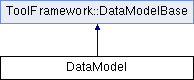
\includegraphics[height=2.000000cm]{classDataModel}
\end{center}
\end{figure}
\doxysubsection*{Public Member Functions}
\begin{DoxyCompactItemize}
\item 
\mbox{\Hypertarget{classDataModel_abff03aef2cb531142a35781bb87c3365}\label{classDataModel_abff03aef2cb531142a35781bb87c3365}} 
\mbox{\hyperlink{classDataModel_abff03aef2cb531142a35781bb87c3365}{Data\+Model}} ()
\begin{DoxyCompactList}\small\item\em Simple constructor. \end{DoxyCompactList}\end{DoxyCompactItemize}
\doxysubsection*{Additional Inherited Members}


\doxysubsection{Detailed Description}
This class Is a transient data model class for your Tools within the Tool\+Chain. If Tools need to comunicate they pass all data objects through the data model. There fore inter tool data objects should be deffined in this class.

\begin{DoxyParagraph}{Author}
B.\+Richards 
\end{DoxyParagraph}
\begin{DoxyParagraph}{Date}
2019/05/26 18\+:34\+:00 
\end{DoxyParagraph}


The documentation for this class was generated from the following files\+:\begin{DoxyCompactItemize}
\item 
Data\+Model/Data\+Model.\+h\item 
Data\+Model/Data\+Model.\+cpp\end{DoxyCompactItemize}

\hypertarget{classDummyTool}{}\doxysection{Dummy\+Tool Class Reference}
\label{classDummyTool}\index{DummyTool@{DummyTool}}


{\ttfamily \#include $<$Dummy\+Tool.\+h$>$}

Inheritance diagram for Dummy\+Tool\+:\begin{figure}[H]
\begin{center}
\leavevmode
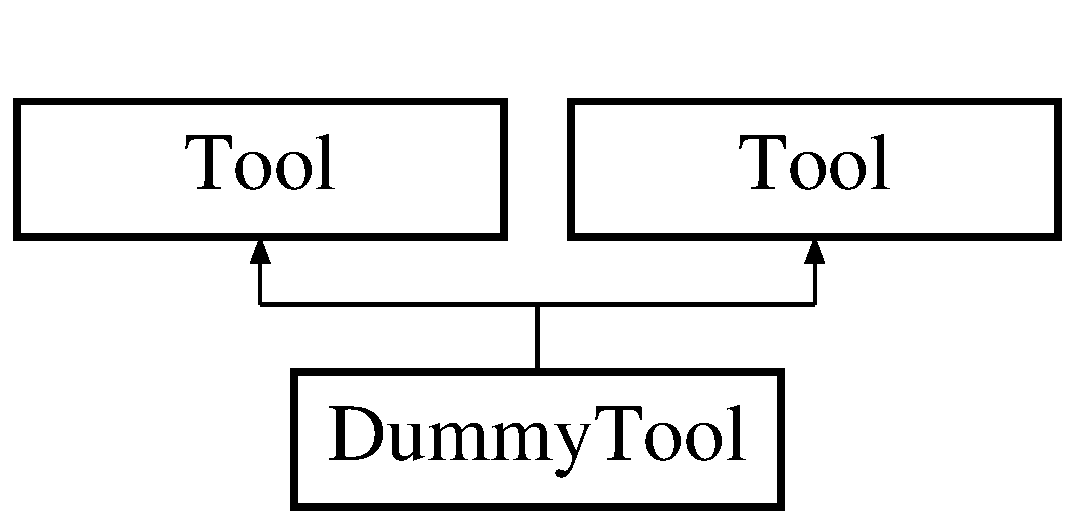
\includegraphics[height=2.000000cm]{classDummyTool}
\end{center}
\end{figure}
\doxysubsection*{Public Member Functions}
\begin{DoxyCompactItemize}
\item 
\mbox{\Hypertarget{classDummyTool_a33914471b4de346168aa92b5febb6f9c}\label{classDummyTool_a33914471b4de346168aa92b5febb6f9c}} 
\mbox{\hyperlink{classDummyTool_a33914471b4de346168aa92b5febb6f9c}{Dummy\+Tool}} ()
\begin{DoxyCompactList}\small\item\em Constructor. \end{DoxyCompactList}\item 
\mbox{\Hypertarget{classDummyTool_a0d9cd781681a06ee3cf0cd1e7bb770a8}\label{classDummyTool_a0d9cd781681a06ee3cf0cd1e7bb770a8}} 
bool \mbox{\hyperlink{classDummyTool_a0d9cd781681a06ee3cf0cd1e7bb770a8}{Initialise}} (std\+::string configfile, \mbox{\hyperlink{classDataModel}{Data\+Model}} \&data)
\begin{DoxyCompactList}\small\item\em Assigns verbosity from config file and creates a log message. \end{DoxyCompactList}\item 
\mbox{\Hypertarget{classDummyTool_ac107b31f1785c1cc803e0e65be548047}\label{classDummyTool_ac107b31f1785c1cc803e0e65be548047}} 
bool \mbox{\hyperlink{classDummyTool_ac107b31f1785c1cc803e0e65be548047}{Execute}} ()
\begin{DoxyCompactList}\small\item\em Creates a log message. \end{DoxyCompactList}\item 
\mbox{\Hypertarget{classDummyTool_aacb5d0b9906a27c2b4bba4aae9bc093a}\label{classDummyTool_aacb5d0b9906a27c2b4bba4aae9bc093a}} 
bool \mbox{\hyperlink{classDummyTool_aacb5d0b9906a27c2b4bba4aae9bc093a}{Finalise}} ()
\begin{DoxyCompactList}\small\item\em Does nothing. \end{DoxyCompactList}\end{DoxyCompactItemize}
\doxysubsection*{Additional Inherited Members}


\doxysubsection{Detailed Description}
This is a simple dummy \mbox{\hyperlink{classTool}{Tool}} designed to show operation of a \mbox{\hyperlink{classTool}{Tool}}. It also provides a default \mbox{\hyperlink{classTool}{Tool}} for the Default \mbox{\hyperlink{classToolChain}{Tool\+Chain}}.

\begin{DoxyParagraph}{Author}
B.\+Richards 
\end{DoxyParagraph}
\begin{DoxyParagraph}{Date}
2019/05/28 10\+:44\+:00 
\end{DoxyParagraph}


The documentation for this class was generated from the following files\+:\begin{DoxyCompactItemize}
\item 
User\+Tools/\+Dummy\+Tool/Dummy\+Tool.\+h\item 
User\+Tools/\+Dummy\+Tool/Dummy\+Tool.\+cpp\end{DoxyCompactItemize}

\hypertarget{classLogger}{\section{Logger Class Reference}
\label{classLogger}\index{Logger@{Logger}}
}


{\ttfamily \#include $<$Logger.\-h$>$}

Inheritance diagram for Logger\-:\begin{figure}[H]
\begin{center}
\leavevmode
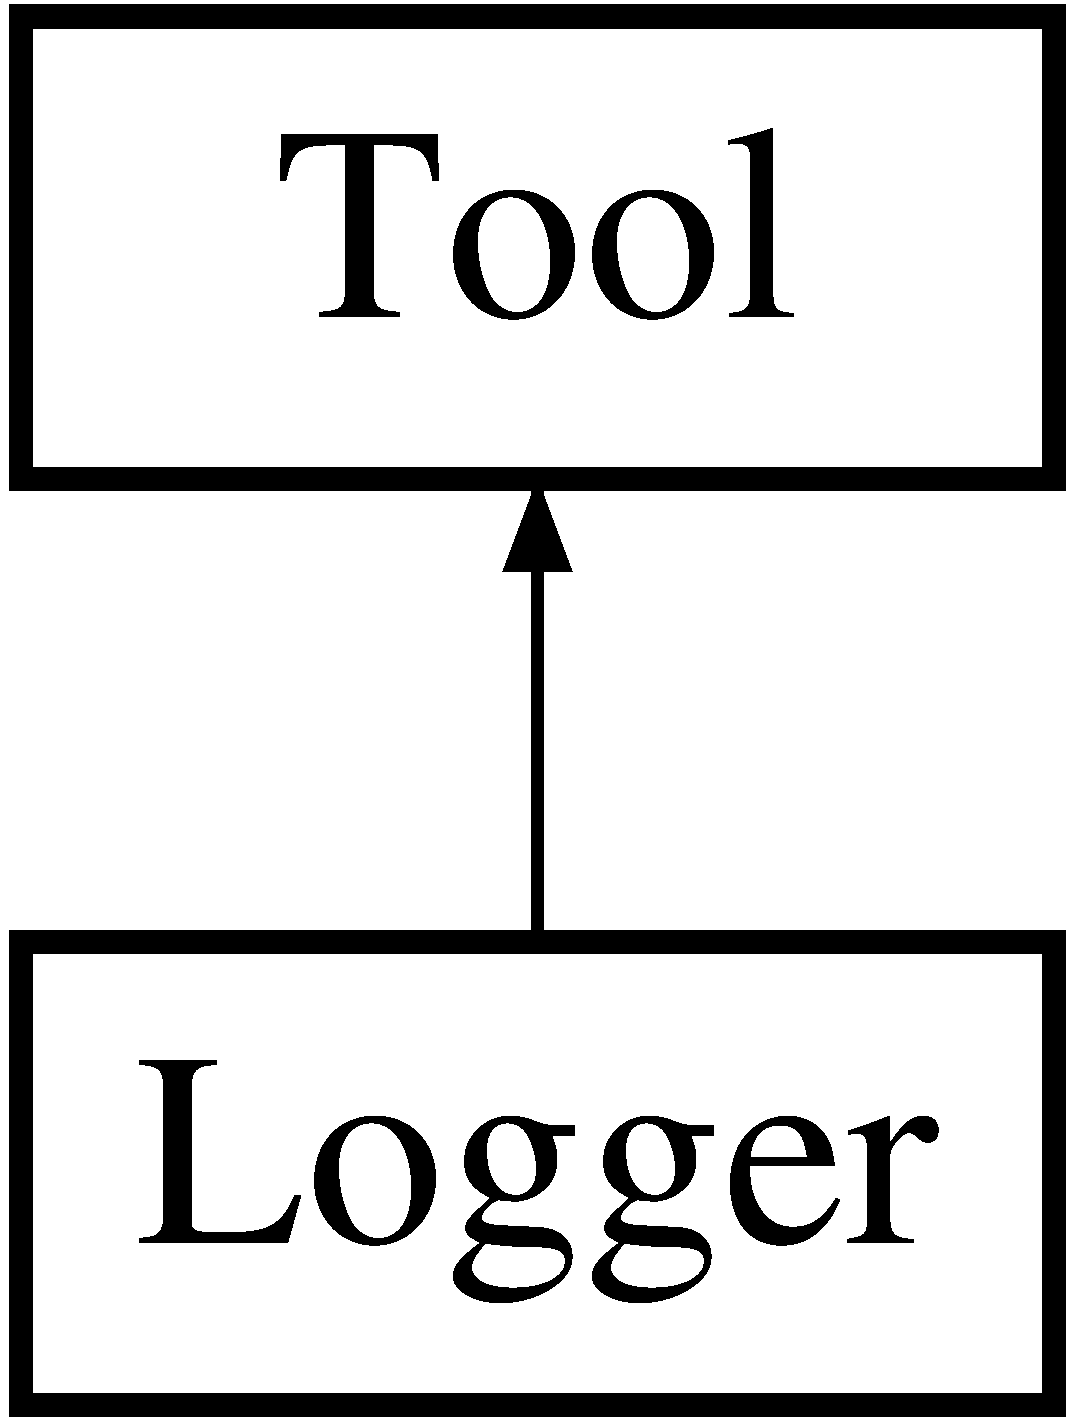
\includegraphics[height=2.000000cm]{classLogger}
\end{center}
\end{figure}
\subsection*{Public Member Functions}
\begin{DoxyCompactItemize}
\item 
\hypertarget{classLogger_abc41bfb031d896170c7675fa96a6b30c}{\hyperlink{classLogger_abc41bfb031d896170c7675fa96a6b30c}{Logger} ()}\label{classLogger_abc41bfb031d896170c7675fa96a6b30c}

\begin{DoxyCompactList}\small\item\em Construtor. \end{DoxyCompactList}\item 
\hypertarget{classLogger_a1b598f35f454e24f9e9abc9f18c3e98f}{bool \hyperlink{classLogger_a1b598f35f454e24f9e9abc9f18c3e98f}{Initialise} (std\-::string configfile, \hyperlink{classDataModel}{Data\-Model} \&data)}\label{classLogger_a1b598f35f454e24f9e9abc9f18c3e98f}

\begin{DoxyCompactList}\small\item\em Sets up a Z\-M\-Q\-\_\-\-P\-U\-L\-L socket which on the log part form the config file. \end{DoxyCompactList}\item 
\hypertarget{classLogger_a140ebede2975159a5abe7c59e56ec0ec}{bool \hyperlink{classLogger_a140ebede2975159a5abe7c59e56ec0ec}{Execute} ()}\label{classLogger_a140ebede2975159a5abe7c59e56ec0ec}

\begin{DoxyCompactList}\small\item\em Listens on socket for logging message printing them to screen when received. \end{DoxyCompactList}\item 
\hypertarget{classLogger_a2c70367a86d5999db21324ccb58f44ed}{bool \hyperlink{classLogger_a2c70367a86d5999db21324ccb58f44ed}{Finalise} ()}\label{classLogger_a2c70367a86d5999db21324ccb58f44ed}

\begin{DoxyCompactList}\small\item\em Closes socket and cleans up. \end{DoxyCompactList}\end{DoxyCompactItemize}
\subsection*{Additional Inherited Members}


\subsection{Detailed Description}
This is a demonstration tool that can receive \hyperlink{classLogging}{Logging} messages from Tool\-Chains

\begin{DoxyParagraph}{Author\-:}
B.\-Richards 
\end{DoxyParagraph}
\begin{DoxyParagraph}{Date\-:}
2019/05/28 10\-:44\-:00 
\end{DoxyParagraph}
Contact\-: \href{mailto:b.richards@qmul.ac.uk}{\tt b.\-richards@qmul.\-ac.\-uk} 

The documentation for this class was generated from the following files\-:\begin{DoxyCompactItemize}
\item 
User\-Tools/\-Logger/Logger.\-h\item 
User\-Tools/\-Logger/Logger.\-cpp\end{DoxyCompactItemize}

\hypertarget{classLogging}{\section{Logging Class Reference}
\label{classLogging}\index{Logging@{Logging}}
}


{\ttfamily \#include $<$Logging.\-h$>$}

Inheritance diagram for Logging\-:\begin{figure}[H]
\begin{center}
\leavevmode
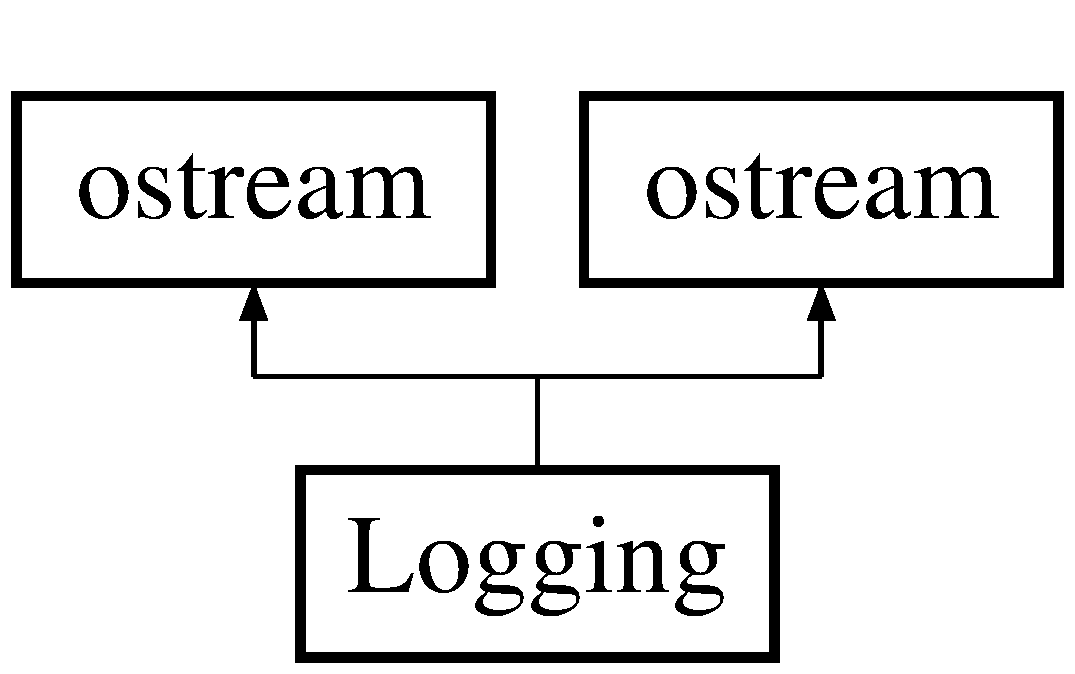
\includegraphics[height=2.000000cm]{classLogging}
\end{center}
\end{figure}
\subsection*{Public Member Functions}
\begin{DoxyCompactItemize}
\item 
\hyperlink{classLogging_ae7cc7299c697019f273b75cbfefff848}{Logging} (std\-::ostream \&str, zmq\-::context\-\_\-t $\ast$context, boost\-::uuids\-::uuid U\-U\-I\-D, std\-::string service, std\-::string mode, std\-::string localpath=\char`\"{}\char`\"{}, std\-::string logservice=\char`\"{}\char`\"{}, int logport=0)
\item 
{\footnotesize template$<$typename T $>$ }\\void \hyperlink{classLogging_af7839ee68729b066da269cc012b1fcc9}{Log} (T message, int messagelevel=1, int verbose=1)
\item 
bool \hyperlink{classLogging_a7a0c89c152ad81fb41a849ed9d81e429}{Change\-Out\-File} (std\-::string localpath)
\end{DoxyCompactItemize}
\subsection*{Public Attributes}
\begin{DoxyCompactItemize}
\item 
\hypertarget{classLogging_a9622376d4c126c163334149cabc98bcc}{My\-Stream\-Buf \hyperlink{classLogging_a9622376d4c126c163334149cabc98bcc}{buffer}}\label{classLogging_a9622376d4c126c163334149cabc98bcc}

\begin{DoxyCompactList}\small\item\em Stream buffer used to replace std\-::cout for redirection to coustom output. \end{DoxyCompactList}\end{DoxyCompactItemize}


\subsection{Detailed Description}
This class handels the logging, which can be directed to screen or file or over the via the \hyperlink{classToolChain}{Tool\-Chain} Config file

\begin{DoxyParagraph}{Author\-:}
B.\-Richards 
\end{DoxyParagraph}
\begin{DoxyParagraph}{Date\-:}
2019/05/27 18\-:34\-:00 
\end{DoxyParagraph}
Contact\-: \href{mailto:b.richards@qmul.ac.uk}{\tt b.\-richards@qmul.\-ac.\-uk} 

\subsection{Constructor \& Destructor Documentation}
\hypertarget{classLogging_ae7cc7299c697019f273b75cbfefff848}{\index{Logging@{Logging}!Logging@{Logging}}
\index{Logging@{Logging}!Logging@{Logging}}
\subsubsection[{Logging}]{\setlength{\rightskip}{0pt plus 5cm}Logging\-::\-Logging (
\begin{DoxyParamCaption}
\item[{std\-::ostream \&}]{str, }
\item[{zmq\-::context\-\_\-t $\ast$}]{context, }
\item[{boost\-::uuids\-::uuid}]{U\-U\-I\-D, }
\item[{std\-::string}]{service, }
\item[{std\-::string}]{mode, }
\item[{std\-::string}]{localpath = {\ttfamily \char`\"{}\char`\"{}}, }
\item[{std\-::string}]{logservice = {\ttfamily \char`\"{}\char`\"{}}, }
\item[{int}]{logport = {\ttfamily 0}}
\end{DoxyParamCaption}
)\hspace{0.3cm}{\ttfamily [inline]}}}\label{classLogging_ae7cc7299c697019f273b75cbfefff848}
Constructor for \hyperlink{classLogging}{Logging} class


\begin{DoxyParams}{Parameters}
{\em str} & \\
\hline
{\em context} & Pointer to Z\-M\-W context used for creating sockets \\
\hline
{\em U\-U\-I\-D} & \hyperlink{classToolChain}{Tool\-Chain} U\-U\-I\-D for unique labelling of log messages \\
\hline
{\em service} & \\
\hline
{\em mode} & \\
\hline
{\em localpath} & Local path for log output file \\
\hline
{\em logservice} & Remote service to connect to to send logs \\
\hline
{\em logport} & remothe port to send logging information to \\
\hline
\end{DoxyParams}


\subsection{Member Function Documentation}
\hypertarget{classLogging_a7a0c89c152ad81fb41a849ed9d81e429}{\index{Logging@{Logging}!Change\-Out\-File@{Change\-Out\-File}}
\index{Change\-Out\-File@{Change\-Out\-File}!Logging@{Logging}}
\subsubsection[{Change\-Out\-File}]{\setlength{\rightskip}{0pt plus 5cm}bool Logging\-::\-Change\-Out\-File (
\begin{DoxyParamCaption}
\item[{std\-::string}]{localpath}
\end{DoxyParamCaption}
)\hspace{0.3cm}{\ttfamily [inline]}}}\label{classLogging_a7a0c89c152ad81fb41a849ed9d81e429}
Functionn to change the logs out file if set to a local path.


\begin{DoxyParams}{Parameters}
{\em localpath} & path to new log file. \\
\hline
\end{DoxyParams}
\begin{DoxyReturn}{Returns}
value is bool success of opening new logfile. 
\end{DoxyReturn}
\hypertarget{classLogging_af7839ee68729b066da269cc012b1fcc9}{\index{Logging@{Logging}!Log@{Log}}
\index{Log@{Log}!Logging@{Logging}}
\subsubsection[{Log}]{\setlength{\rightskip}{0pt plus 5cm}template$<$typename T $>$ void Logging\-::\-Log (
\begin{DoxyParamCaption}
\item[{T}]{message, }
\item[{int}]{messagelevel = {\ttfamily 1}, }
\item[{int}]{verbose = {\ttfamily 1}}
\end{DoxyParamCaption}
)\hspace{0.3cm}{\ttfamily [inline]}}}\label{classLogging_af7839ee68729b066da269cc012b1fcc9}
Function to create a log messages.


\begin{DoxyParams}{Parameters}
{\em message} & templated log message text. \\
\hline
{\em messagelevel} & message verbosity level of the message being sent (e.\-g. if 'messagelevel$>$= verbose' Then message is sent). \\
\hline
{\em verbose} & verbosity level of the current \hyperlink{classTool}{Tool}. \\
\hline
\end{DoxyParams}


The documentation for this class was generated from the following file\-:\begin{DoxyCompactItemize}
\item 
src/\-Logging/Logging.\-h\end{DoxyCompactItemize}

\hypertarget{structLogging__thread__args}{\section{Logging\-\_\-thread\-\_\-args Struct Reference}
\label{structLogging__thread__args}\index{Logging\-\_\-thread\-\_\-args@{Logging\-\_\-thread\-\_\-args}}
}


{\ttfamily \#include $<$Logging.\-h$>$}

\subsection*{Public Member Functions}
\begin{DoxyCompactItemize}
\item 
\hypertarget{structLogging__thread__args_a9496cec11539e17b104d3cbdf3174fdb}{\hyperlink{structLogging__thread__args_a9496cec11539e17b104d3cbdf3174fdb}{Logging\-\_\-thread\-\_\-args} (zmq\-::context\-\_\-t $\ast$incontext, boost\-::uuids\-::uuid in\-U\-U\-I\-D, std\-::string inlogservice, int inlogport)}\label{structLogging__thread__args_a9496cec11539e17b104d3cbdf3174fdb}

\begin{DoxyCompactList}\small\item\em Simple constructor to assign thread variables. \end{DoxyCompactList}\end{DoxyCompactItemize}
\subsection*{Public Attributes}
\begin{DoxyCompactItemize}
\item 
\hypertarget{structLogging__thread__args_addacf7a55861c13832a75b88d74c006c}{zmq\-::context\-\_\-t $\ast$ \hyperlink{structLogging__thread__args_addacf7a55861c13832a75b88d74c006c}{context}}\label{structLogging__thread__args_addacf7a55861c13832a75b88d74c006c}

\begin{DoxyCompactList}\small\item\em pointer to Z\-M\-Q context for socket creation \end{DoxyCompactList}\item 
\hypertarget{structLogging__thread__args_a3a7c5617b7fa5214c6da407a23266d57}{boost\-::uuids\-::uuid \hyperlink{structLogging__thread__args_a3a7c5617b7fa5214c6da407a23266d57}{U\-U\-I\-D}}\label{structLogging__thread__args_a3a7c5617b7fa5214c6da407a23266d57}

\begin{DoxyCompactList}\small\item\em \hyperlink{classToolChain}{Tool\-Chain} U\-U\-I\-D for unique labelling of log messages. \end{DoxyCompactList}\item 
\hypertarget{structLogging__thread__args_a5a8e255209f5c171a7fbd78f0e308087}{std\-::string \hyperlink{structLogging__thread__args_a5a8e255209f5c171a7fbd78f0e308087}{logservice}}\label{structLogging__thread__args_a5a8e255209f5c171a7fbd78f0e308087}

\begin{DoxyCompactList}\small\item\em Remote service name to connect to. \end{DoxyCompactList}\item 
\hypertarget{structLogging__thread__args_ad5ab1c21e226a694c7f813bcb3ef9002}{int \hyperlink{structLogging__thread__args_ad5ab1c21e226a694c7f813bcb3ef9002}{logport}}\label{structLogging__thread__args_ad5ab1c21e226a694c7f813bcb3ef9002}

\begin{DoxyCompactList}\small\item\em Port to connect to to send remote logging information. \end{DoxyCompactList}\end{DoxyCompactItemize}


\subsection{Detailed Description}
This struct holds the initalisation variables to be passed to the logging thread.

\begin{DoxyParagraph}{Author\-:}
B.\-Richards 
\end{DoxyParagraph}
\begin{DoxyParagraph}{Date\-:}
2019/05/27 18\-:34\-:00 
\end{DoxyParagraph}
Contact\-: \href{mailto:b.richards@qmul.ac.uk}{\tt b.\-richards@qmul.\-ac.\-uk} 

The documentation for this struct was generated from the following file\-:\begin{DoxyCompactItemize}
\item 
src/\-Logging/Logging.\-h\end{DoxyCompactItemize}

\hypertarget{classMyTool}{}\doxysection{My\+Tool Class Reference}
\label{classMyTool}\index{MyTool@{MyTool}}


{\ttfamily \#include $<$My\+Tool.\+h$>$}

Inheritance diagram for My\+Tool\+:\begin{figure}[H]
\begin{center}
\leavevmode
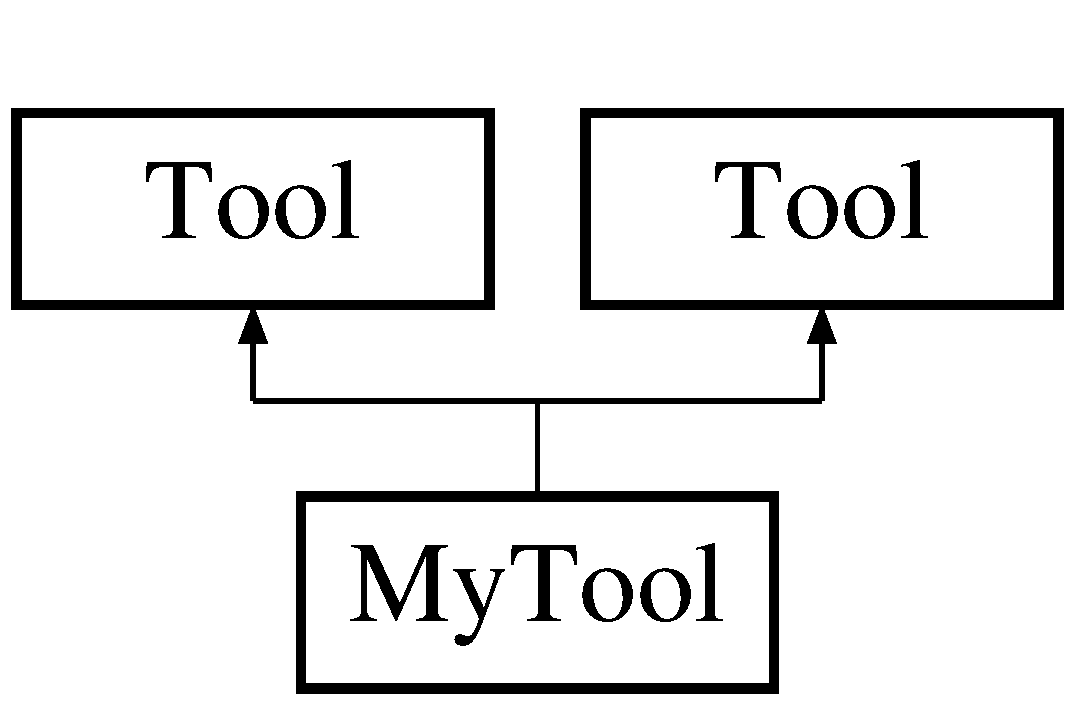
\includegraphics[height=2.000000cm]{classMyTool}
\end{center}
\end{figure}
\doxysubsection*{Public Member Functions}
\begin{DoxyCompactItemize}
\item 
\mbox{\Hypertarget{classMyTool_ad85b796bdd675ae22e69cf40fe7b6314}\label{classMyTool_ad85b796bdd675ae22e69cf40fe7b6314}} 
\mbox{\hyperlink{classMyTool_ad85b796bdd675ae22e69cf40fe7b6314}{My\+Tool}} ()
\begin{DoxyCompactList}\small\item\em Simple constructor. \end{DoxyCompactList}\item 
bool \mbox{\hyperlink{classMyTool_a3bf60061195a18542c4cfb2916b9dad9}{Initialise}} (std\+::string configfile, \mbox{\hyperlink{classDataModel}{Data\+Model}} \&data)
\begin{DoxyCompactList}\small\item\em Initialise Function for setting up Tool resorces. \end{DoxyCompactList}\item 
\mbox{\Hypertarget{classMyTool_a0a58122023af90b9200d0e71e89cfb36}\label{classMyTool_a0a58122023af90b9200d0e71e89cfb36}} 
bool \mbox{\hyperlink{classMyTool_a0a58122023af90b9200d0e71e89cfb36}{Execute}} ()
\begin{DoxyCompactList}\small\item\em Executre function used to perform Tool perpose. \end{DoxyCompactList}\item 
\mbox{\Hypertarget{classMyTool_a060ec6356451aa335d0de41093c9992f}\label{classMyTool_a060ec6356451aa335d0de41093c9992f}} 
bool \mbox{\hyperlink{classMyTool_a060ec6356451aa335d0de41093c9992f}{Finalise}} ()
\begin{DoxyCompactList}\small\item\em Finalise funciton used to clean up resorces. \end{DoxyCompactList}\end{DoxyCompactItemize}
\doxysubsection*{Additional Inherited Members}


\doxysubsection{Detailed Description}
This is a balnk template for a Tool used by the script to generate a new custom tool. Please fill out the descripton and author information.

\begin{DoxyParagraph}{Author}
B.\+Richards 
\end{DoxyParagraph}
\begin{DoxyParagraph}{Date}
2019/05/28 10\+:44\+:00 
\end{DoxyParagraph}


\doxysubsection{Member Function Documentation}
\mbox{\Hypertarget{classMyTool_a3bf60061195a18542c4cfb2916b9dad9}\label{classMyTool_a3bf60061195a18542c4cfb2916b9dad9}} 
\index{MyTool@{MyTool}!Initialise@{Initialise}}
\index{Initialise@{Initialise}!MyTool@{MyTool}}
\doxysubsubsection{\texorpdfstring{Initialise()}{Initialise()}}
{\footnotesize\ttfamily bool My\+Tool\+::\+Initialise (\begin{DoxyParamCaption}\item[{std\+::string}]{configfile,  }\item[{\mbox{\hyperlink{classDataModel}{Data\+Model}} \&}]{data }\end{DoxyParamCaption})\hspace{0.3cm}{\ttfamily [virtual]}}



Initialise Function for setting up Tool resorces. 


\begin{DoxyParams}{Parameters}
{\em configfile} & The path and name of the dynamic configuration file to read in.\\
\hline
{\em data} & A reference to the transient data class used to pass information between Tools. \\
\hline
\end{DoxyParams}


Implements \mbox{\hyperlink{classToolFramework_1_1Tool_acd45ac0abe3bf8b2cfbdd78802e2c648}{Tool\+Framework\+::\+Tool}}.



The documentation for this class was generated from the following files\+:\begin{DoxyCompactItemize}
\item 
User\+Tools/template/My\+Tool.\+h\item 
User\+Tools/template/My\+Tool.\+cpp\end{DoxyCompactItemize}

\hypertarget{classPointerWrapper}{}\doxysection{Pointer\+Wrapper$<$ T $>$ Class Template Reference}
\label{classPointerWrapper}\index{PointerWrapper$<$ T $>$@{PointerWrapper$<$ T $>$}}


{\ttfamily \#include $<$Pointer\+Wrapper.\+h$>$}

Inheritance diagram for Pointer\+Wrapper$<$ T $>$\+:\begin{figure}[H]
\begin{center}
\leavevmode
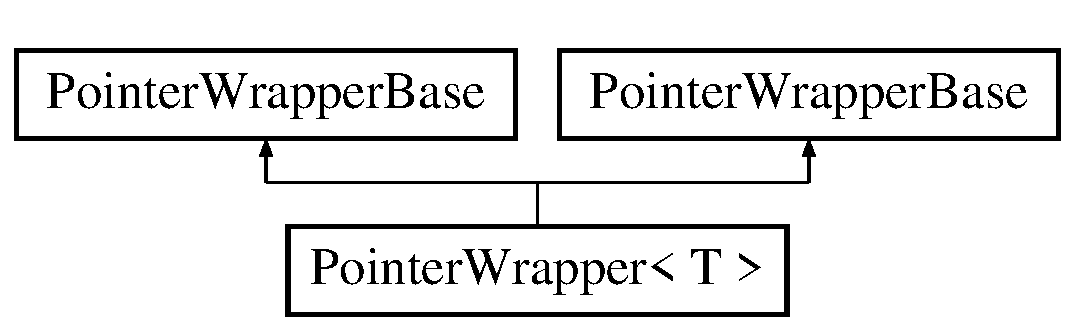
\includegraphics[height=2.000000cm]{classPointerWrapper}
\end{center}
\end{figure}
\doxysubsection*{Public Member Functions}
\begin{DoxyCompactItemize}
\item 
\mbox{\hyperlink{classPointerWrapper_aa645eb1963f91c9bddf5fd6ff578751b}{Pointer\+Wrapper}} (T $\ast$inpointer)
\begin{DoxyCompactList}\small\item\em Constructor. \end{DoxyCompactList}\end{DoxyCompactItemize}
\doxysubsection*{Public Attributes}
\begin{DoxyCompactItemize}
\item 
\mbox{\Hypertarget{classPointerWrapper_a4866798d33eed0a9aeaa3bcda53c4a0d}\label{classPointerWrapper_a4866798d33eed0a9aeaa3bcda53c4a0d}} 
T $\ast$ \mbox{\hyperlink{classPointerWrapper_a4866798d33eed0a9aeaa3bcda53c4a0d}{pointer}}
\begin{DoxyCompactList}\small\item\em Pointer to the orignial obkect. \end{DoxyCompactList}\end{DoxyCompactItemize}


\doxysubsection{Detailed Description}
\subsubsection*{template$<$class T$>$\newline
class Pointer\+Wrapper$<$ T $>$}

Teplated derived class of \mbox{\hyperlink{classPointerWrapperBase}{Pointer\+Wrapper\+Base}} to provide a plymorphic interface to stored poitner variables.

\begin{DoxyParagraph}{Author}
B.\+Richards 
\end{DoxyParagraph}
\begin{DoxyParagraph}{Date}
2019/05/28 10\+:44\+:00 
\end{DoxyParagraph}


\doxysubsection{Constructor \& Destructor Documentation}
\mbox{\Hypertarget{classPointerWrapper_aa645eb1963f91c9bddf5fd6ff578751b}\label{classPointerWrapper_aa645eb1963f91c9bddf5fd6ff578751b}} 
\index{PointerWrapper$<$ T $>$@{PointerWrapper$<$ T $>$}!PointerWrapper@{PointerWrapper}}
\index{PointerWrapper@{PointerWrapper}!PointerWrapper$<$ T $>$@{PointerWrapper$<$ T $>$}}
\doxysubsubsection{\texorpdfstring{PointerWrapper()}{PointerWrapper()}}
{\footnotesize\ttfamily template$<$class T $>$ \\
\mbox{\hyperlink{classPointerWrapper}{Pointer\+Wrapper}}$<$ T $>$\+::\mbox{\hyperlink{classPointerWrapper}{Pointer\+Wrapper}} (\begin{DoxyParamCaption}\item[{T $\ast$}]{inpointer }\end{DoxyParamCaption})\hspace{0.3cm}{\ttfamily [inline]}}



Constructor. 


\begin{DoxyParams}{Parameters}
{\em inpointer} & The pointer to be wrapped. \\
\hline
\end{DoxyParams}


The documentation for this class was generated from the following file\+:\begin{DoxyCompactItemize}
\item 
src/\+Store/Pointer\+Wrapper.\+h\end{DoxyCompactItemize}

\hypertarget{classPointerWrapperBase}{\section{Pointer\-Wrapper\-Base Class Reference}
\label{classPointerWrapperBase}\index{Pointer\-Wrapper\-Base@{Pointer\-Wrapper\-Base}}
}


{\ttfamily \#include $<$Pointer\-Wrapper.\-h$>$}

Inheritance diagram for Pointer\-Wrapper\-Base\-:\begin{figure}[H]
\begin{center}
\leavevmode
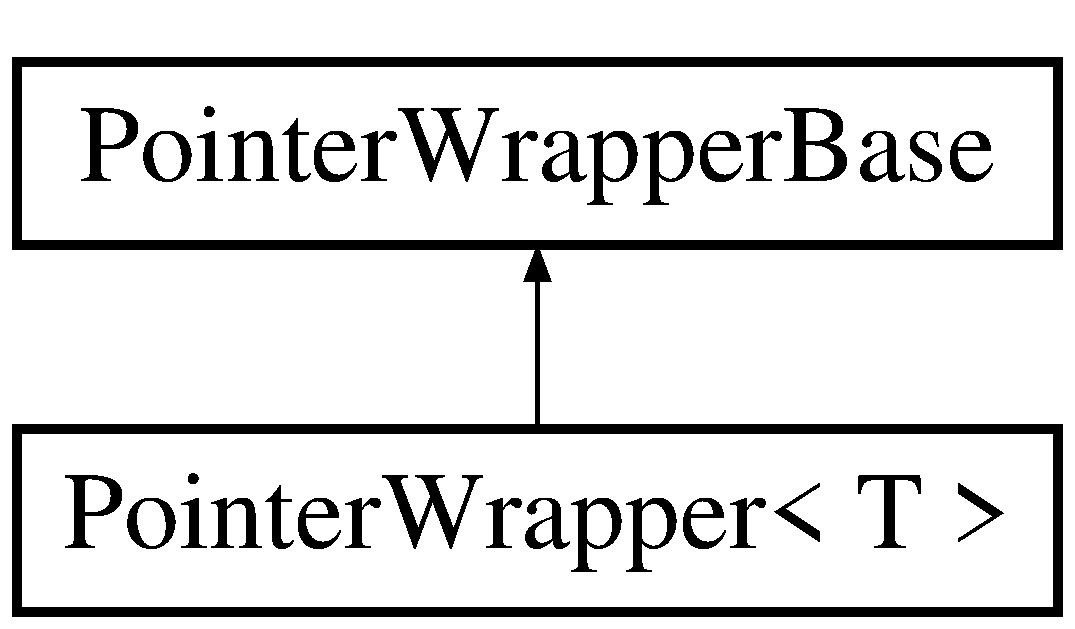
\includegraphics[height=2.000000cm]{classPointerWrapperBase}
\end{center}
\end{figure}
\subsection*{Public Member Functions}
\begin{DoxyCompactItemize}
\item 
\hypertarget{classPointerWrapperBase_ac9e248557a8aa248bcbbadc469c77f52}{\hyperlink{classPointerWrapperBase_ac9e248557a8aa248bcbbadc469c77f52}{Pointer\-Wrapper\-Base} ()}\label{classPointerWrapperBase_ac9e248557a8aa248bcbbadc469c77f52}

\begin{DoxyCompactList}\small\item\em Simple constructor. \end{DoxyCompactList}\item 
\hypertarget{classPointerWrapperBase_a842fb0af38187d71678971452c1e1094}{virtual \hyperlink{classPointerWrapperBase_a842fb0af38187d71678971452c1e1094}{$\sim$\-Pointer\-Wrapper\-Base} ()}\label{classPointerWrapperBase_a842fb0af38187d71678971452c1e1094}

\begin{DoxyCompactList}\small\item\em virtual destructor \end{DoxyCompactList}\end{DoxyCompactItemize}


\subsection{Detailed Description}
This class is used to wrap pointers stored in a Boost\-Store. It gives a generic abstract base class to store pointers under

\begin{DoxyParagraph}{Author\-:}
B.\-Richards 
\end{DoxyParagraph}
\begin{DoxyParagraph}{Date\-:}
2019/05/28 10\-:44\-:00 
\end{DoxyParagraph}


The documentation for this class was generated from the following file\-:\begin{DoxyCompactItemize}
\item 
src/\-Store/Pointer\-Wrapper.\-h\end{DoxyCompactItemize}

\hypertarget{classSerialisableObject}{\section{Serialisable\-Object Class Reference}
\label{classSerialisableObject}\index{Serialisable\-Object@{Serialisable\-Object}}
}


{\ttfamily \#include $<$Serialisable\-Object.\-h$>$}

Inheritance diagram for Serialisable\-Object\-:\begin{figure}[H]
\begin{center}
\leavevmode
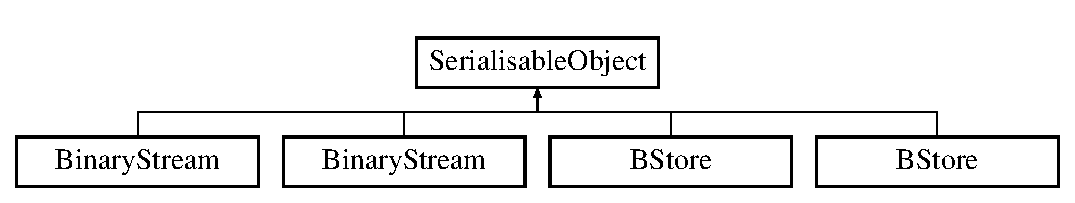
\includegraphics[height=2.000000cm]{classSerialisableObject}
\end{center}
\end{figure}
\subsection*{Public Member Functions}
\begin{DoxyCompactItemize}
\item 
\hypertarget{classSerialisableObject_a3783b1798068a4bdc58fe6cdf7f7929b}{bool {\bfseries Serialise\-Wrapper} (\hyperlink{classBinaryStream}{Binary\-Stream} \&bs)}\label{classSerialisableObject_a3783b1798068a4bdc58fe6cdf7f7929b}

\item 
\hypertarget{classSerialisableObject_ab8916a102bc94764f023b1713fb040db}{virtual bool {\bfseries Serialise} (\hyperlink{classBinaryStream}{Binary\-Stream} \&bs)=0}\label{classSerialisableObject_ab8916a102bc94764f023b1713fb040db}

\item 
\hypertarget{classSerialisableObject_a345b21d2a7c869dedd96ad691fc602bd}{virtual std\-::string {\bfseries Get\-Version} ()=0}\label{classSerialisableObject_a345b21d2a7c869dedd96ad691fc602bd}

\item 
\hypertarget{classSerialisableObject_a9055c98969917d4c652eefdc924b6b75}{virtual bool \hyperlink{classSerialisableObject_a9055c98969917d4c652eefdc924b6b75}{Print} ()=0}\label{classSerialisableObject_a9055c98969917d4c652eefdc924b6b75}

\begin{DoxyCompactList}\small\item\em Simple virtual Pritn function to ensure inhereted classes have one. \end{DoxyCompactList}\end{DoxyCompactItemize}


\subsection{Detailed Description}
An abstract base class for sustom calsses to inherit from to ensure version and type information are present, as well as a Print function and some form of sereialisation.

\begin{DoxyParagraph}{Author\-:}
B.\-Richards 
\end{DoxyParagraph}
\begin{DoxyParagraph}{Date\-:}
2019/05/28 10\-:44\-:00 
\end{DoxyParagraph}


The documentation for this class was generated from the following files\-:\begin{DoxyCompactItemize}
\item 
src/\-Store/Serialisable\-Object.\-h\item 
src/\-Store/Binary\-Stream.\-cpp\end{DoxyCompactItemize}

\hypertarget{classServiceAdd}{\section{Service\-Add Class Reference}
\label{classServiceAdd}\index{Service\-Add@{Service\-Add}}
}


{\ttfamily \#include $<$Service\-Add.\-h$>$}

Inheritance diagram for Service\-Add\-:\begin{figure}[H]
\begin{center}
\leavevmode
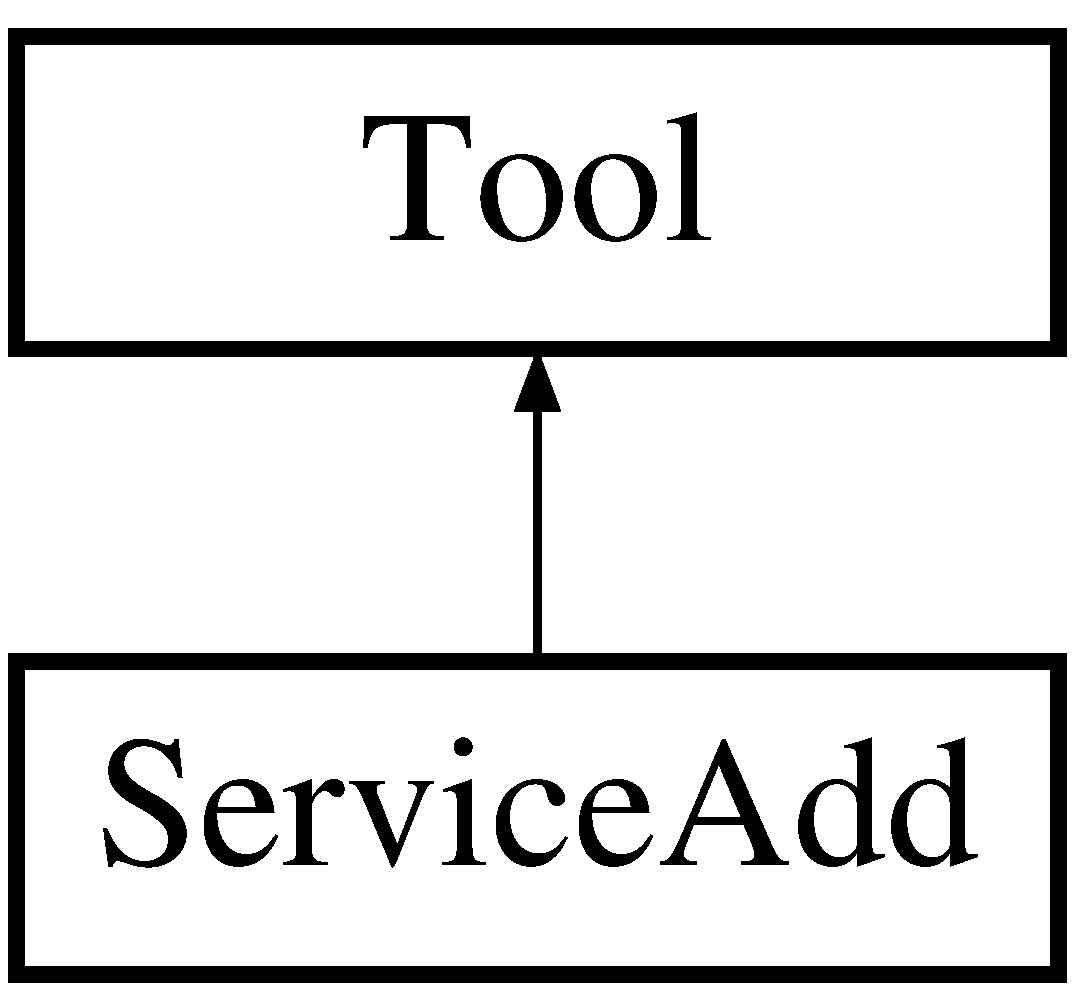
\includegraphics[height=2.000000cm]{classServiceAdd}
\end{center}
\end{figure}
\subsection*{Public Member Functions}
\begin{DoxyCompactItemize}
\item 
\hypertarget{classServiceAdd_a0148b0e038f4b0dd6f12c87cdf233f69}{\hyperlink{classServiceAdd_a0148b0e038f4b0dd6f12c87cdf233f69}{Service\-Add} ()}\label{classServiceAdd_a0148b0e038f4b0dd6f12c87cdf233f69}

\begin{DoxyCompactList}\small\item\em Constrcutor. \end{DoxyCompactList}\item 
\hypertarget{classServiceAdd_a047e44c3d209591703b0bdec1b1b51cd}{bool \hyperlink{classServiceAdd_a047e44c3d209591703b0bdec1b1b51cd}{Initialise} (std\-::string configfile, \hyperlink{classDataModel}{Data\-Model} \&data)}\label{classServiceAdd_a047e44c3d209591703b0bdec1b1b51cd}

\begin{DoxyCompactList}\small\item\em Opens socket to service discoverypublisher and adds a service and assosiated port to broadcast. \end{DoxyCompactList}\item 
\hypertarget{classServiceAdd_a4908df063074b02e73e589d9f07998ac}{bool \hyperlink{classServiceAdd_a4908df063074b02e73e589d9f07998ac}{Execute} ()}\label{classServiceAdd_a4908df063074b02e73e589d9f07998ac}

\begin{DoxyCompactList}\small\item\em Does nothing. \end{DoxyCompactList}\item 
\hypertarget{classServiceAdd_a2e4d3854bcd490935e6e9d39597c7204}{bool \hyperlink{classServiceAdd_a2e4d3854bcd490935e6e9d39597c7204}{Finalise} ()}\label{classServiceAdd_a2e4d3854bcd490935e6e9d39597c7204}

\begin{DoxyCompactList}\small\item\em Opens new connection to service discovery publish thread and removes service from service list. \end{DoxyCompactList}\end{DoxyCompactItemize}
\subsection*{Additional Inherited Members}


\subsection{Detailed Description}
This Tools demonstraits how to add services and publicise connections for them in the Tool\-Cahins multicast beacons.

\begin{DoxyParagraph}{Author\-:}
B.\-Richards 
\end{DoxyParagraph}
\begin{DoxyParagraph}{Date\-:}
2019/05/28 10\-:44\-:00 
\end{DoxyParagraph}
Contact\-: \href{mailto:b.richards@qmul.ac.uk}{\tt b.\-richards@qmul.\-ac.\-uk} 

The documentation for this class was generated from the following files\-:\begin{DoxyCompactItemize}
\item 
User\-Tools/\-Service\-Add/Service\-Add.\-h\item 
User\-Tools/\-Service\-Add/Service\-Add.\-cpp\end{DoxyCompactItemize}

\hypertarget{classServiceDiscovery}{\section{Service\-Discovery Class Reference}
\label{classServiceDiscovery}\index{Service\-Discovery@{Service\-Discovery}}
}


{\ttfamily \#include $<$Service\-Discovery.\-h$>$}

\subsection*{Public Member Functions}
\begin{DoxyCompactItemize}
\item 
\hyperlink{classServiceDiscovery_ab69c2cacaf5a388fac88e57f3361b576}{Service\-Discovery} (bool Send, bool Receive, int remoteport, std\-::string address, int multicastport, zmq\-::context\-\_\-t $\ast$incontext, boost\-::uuids\-::uuid U\-U\-I\-D, std\-::string service, int pubsec=5, int kicksec=60)
\item 
\hyperlink{classServiceDiscovery_a3dbd15f19345b0c9746731308e26b034}{Service\-Discovery} (std\-::string address, int multicastport, zmq\-::context\-\_\-t $\ast$incontext, int kicksec=60)
\item 
\hypertarget{classServiceDiscovery_aee64ecb3b4c07b7f2a070a66ecb7dc70}{\hyperlink{classServiceDiscovery_aee64ecb3b4c07b7f2a070a66ecb7dc70}{$\sim$\-Service\-Discovery} ()}\label{classServiceDiscovery_aee64ecb3b4c07b7f2a070a66ecb7dc70}

\begin{DoxyCompactList}\small\item\em Simple destructor. \end{DoxyCompactList}\end{DoxyCompactItemize}


\subsection{Detailed Description}
This class handels the service discovery for the \hyperlink{classToolChain}{Tool\-Chain}. It oth handels publishing multicast beacons for the Tool\-Cahin and any other customs services and it collates and maintains a list of other remote services form their multicast beacons that Tools can acess via a Z\-M\-Q port and query.

\begin{DoxyParagraph}{Author\-:}
B.\-Richards 
\end{DoxyParagraph}
\begin{DoxyParagraph}{Date\-:}
2019/05/27 18\-:34\-:00 
\end{DoxyParagraph}
Contact\-: \href{mailto:b.richards@qmul.ac.uk}{\tt b.\-richards@qmul.\-ac.\-uk} 

\subsection{Constructor \& Destructor Documentation}
\hypertarget{classServiceDiscovery_ab69c2cacaf5a388fac88e57f3361b576}{\index{Service\-Discovery@{Service\-Discovery}!Service\-Discovery@{Service\-Discovery}}
\index{Service\-Discovery@{Service\-Discovery}!ServiceDiscovery@{Service\-Discovery}}
\subsubsection[{Service\-Discovery}]{\setlength{\rightskip}{0pt plus 5cm}Service\-Discovery\-::\-Service\-Discovery (
\begin{DoxyParamCaption}
\item[{bool}]{Send, }
\item[{bool}]{Receive, }
\item[{int}]{remoteport, }
\item[{std\-::string}]{address, }
\item[{int}]{multicastport, }
\item[{zmq\-::context\-\_\-t $\ast$}]{incontext, }
\item[{boost\-::uuids\-::uuid}]{U\-U\-I\-D, }
\item[{std\-::string}]{service, }
\item[{int}]{pubsec = {\ttfamily 5}, }
\item[{int}]{kicksec = {\ttfamily 60}}
\end{DoxyParamCaption}
)}}\label{classServiceDiscovery_ab69c2cacaf5a388fac88e57f3361b576}
Constructor for S\-Ervice\-Discovery


\begin{DoxyParams}{Parameters}
{\em Send} & bool to determin if the publish thread is created to send multicast beacons \\
\hline
{\em Receive} & boot to determin if the listen thread is created to receive and collate incomming multicast beacons \\
\hline
{\em remoteport} & Port number to publish for remote connections to control the \hyperlink{classToolChain}{Tool\-Chain} \\
\hline
{\em address} & \\
\hline
{\em multicastport} & Port to use for multicast beacons \\
\hline
{\em incontext} & Pointer to Z\-M\-Q contect for socket creation \\
\hline
{\em U\-U\-I\-D} & Unique U\-U\-I\-D identifier for the \hyperlink{classToolChain}{Tool\-Chain} to be used is service beacons \\
\hline
{\em service} & Name to broadcast to identify the \hyperlink{classToolChain}{Tool\-Chain} type in beacon \\
\hline
{\em pubsec} & The number of seconds between sending multicast beacons \\
\hline
{\em kicksec} & The number of seconds without receiving a beacon from a remote service to remove them from the services list. \\
\hline
\end{DoxyParams}
\hypertarget{classServiceDiscovery_a3dbd15f19345b0c9746731308e26b034}{\index{Service\-Discovery@{Service\-Discovery}!Service\-Discovery@{Service\-Discovery}}
\index{Service\-Discovery@{Service\-Discovery}!ServiceDiscovery@{Service\-Discovery}}
\subsubsection[{Service\-Discovery}]{\setlength{\rightskip}{0pt plus 5cm}Service\-Discovery\-::\-Service\-Discovery (
\begin{DoxyParamCaption}
\item[{std\-::string}]{address, }
\item[{int}]{multicastport, }
\item[{zmq\-::context\-\_\-t $\ast$}]{incontext, }
\item[{int}]{kicksec = {\ttfamily 60}}
\end{DoxyParamCaption}
)}}\label{classServiceDiscovery_a3dbd15f19345b0c9746731308e26b034}
Simpler constructor for only receiving multicast beacons and not sending. This therefor doesnt require the U\-U\-I\-D and plublish variables, so can be used for passive listener.

variables are the same as above. 

The documentation for this class was generated from the following files\-:\begin{DoxyCompactItemize}
\item 
src/\-Service\-Discovery/Service\-Discovery.\-h\item 
src/\-Service\-Discovery/Service\-Discovery.\-cpp\end{DoxyCompactItemize}

\hypertarget{classStore}{}\doxysection{Store Class Reference}
\label{classStore}\index{Store@{Store}}


{\ttfamily \#include $<$Store.\+h$>$}

\doxysubsection*{Public Member Functions}
\begin{DoxyCompactItemize}
\item 
bool \mbox{\hyperlink{classStore_a5247080901fb214804d0191681a30a83}{Initialise}} (std\+::string filename)
\begin{DoxyCompactList}\small\item\em Initialises \mbox{\hyperlink{classStore}{Store}} by reading in entries from an ASCII text file, when each line is a variable and its value in key value pairs. \end{DoxyCompactList}\item 
void \mbox{\hyperlink{classStore_adb84e3fb286cae07f64e8186b7ab04e1}{Json\+Parser}} (std\+::string input)
\begin{DoxyCompactList}\small\item\em Converts a flat JSON formatted string to \mbox{\hyperlink{classStore}{Store}} entries in the form of key value pairs. \end{DoxyCompactList}\item 
\mbox{\Hypertarget{classStore_a9d2f000bd849a9f5de71c3ba62dca340}\label{classStore_a9d2f000bd849a9f5de71c3ba62dca340}} 
void \mbox{\hyperlink{classStore_a9d2f000bd849a9f5de71c3ba62dca340}{Print}} ()
\begin{DoxyCompactList}\small\item\em Prints the contents of the \mbox{\hyperlink{classStore}{Store}}. \end{DoxyCompactList}\item 
\mbox{\Hypertarget{classStore_a7fce0f8f3ec7978c5e7cd3d7053f899b}\label{classStore_a7fce0f8f3ec7978c5e7cd3d7053f899b}} 
void \mbox{\hyperlink{classStore_a7fce0f8f3ec7978c5e7cd3d7053f899b}{Delete}} ()
\begin{DoxyCompactList}\small\item\em Deletes all entries in the \mbox{\hyperlink{classStore}{Store}}. \end{DoxyCompactList}\item 
bool \mbox{\hyperlink{classStore_a41eaa81c4612fb5bdbf850afb6428977}{Has}} (std\+::string key)
\begin{DoxyCompactList}\small\item\em Returns bool based on if store contains entry given by sting. \end{DoxyCompactList}\item 
\mbox{\Hypertarget{classStore_a002824916990f01593ac6806841179c2}\label{classStore_a002824916990f01593ac6806841179c2}} 
std\+::vector$<$ std\+::string $>$ {\bfseries Keys} ()
\item 
{\footnotesize template$<$typename T $>$ }\\bool \mbox{\hyperlink{classStore_abdc0134daa34b808328070f5d6b295f3}{Get}} (std\+::string name, T \&out)
\item 
bool \mbox{\hyperlink{classStore_ac9c263e8556970c385e2630de3a5ea29}{Get}} (std\+::string name, std\+::string \&out)
\item 
{\footnotesize template$<$typename T $>$ }\\T \mbox{\hyperlink{classStore_a26d26db839f734e0af5404b7dac40dae}{Get}} (std\+::string name)
\item 
{\footnotesize template$<$typename T $>$ }\\void \mbox{\hyperlink{classStore_af586739813ce18da6f5e3561d134a814}{Set}} (std\+::string name, T in)
\item 
std\+::string $\ast$ \mbox{\hyperlink{classStore_a790ca02bc7d11648edf0c8d5df3751fe}{operator\mbox{[}$\,$\mbox{]}}} (std\+::string key)
\item 
{\footnotesize template$<$typename T $>$ }\\void \mbox{\hyperlink{classStore_abe9b65d1308c43dc4158b00d6aed7385}{operator$>$$>$}} (T \&obj)
\item 
\mbox{\Hypertarget{classStore_ae4d74118828e6afc0ca1008186d53f92}\label{classStore_ae4d74118828e6afc0ca1008186d53f92}} 
std\+::map$<$ std\+::string, std\+::string $>$\+::const\+\_\+iterator {\bfseries begin} ()
\item 
\mbox{\Hypertarget{classStore_a08f6f8f52c4bded54b78495cefee842a}\label{classStore_a08f6f8f52c4bded54b78495cefee842a}} 
std\+::map$<$ std\+::string, std\+::string $>$\+::const\+\_\+iterator {\bfseries end} ()
\end{DoxyCompactItemize}


\doxysubsection{Detailed Description}
This class Is a dynamic data storeage class and can be used to store variables of any type listed by ASCII key. The storage of the varaible is in ASCII, so is inefficent for large numbers of entries.

\begin{DoxyParagraph}{Author}
B.\+Richards 
\end{DoxyParagraph}
\begin{DoxyParagraph}{Date}
2019/05/28 10\+:44\+:00 
\end{DoxyParagraph}


\doxysubsection{Member Function Documentation}
\mbox{\Hypertarget{classStore_a26d26db839f734e0af5404b7dac40dae}\label{classStore_a26d26db839f734e0af5404b7dac40dae}} 
\index{Store@{Store}!Get@{Get}}
\index{Get@{Get}!Store@{Store}}
\doxysubsubsection{\texorpdfstring{Get()}{Get()}\hspace{0.1cm}{\footnotesize\ttfamily [1/3]}}
{\footnotesize\ttfamily template$<$typename T $>$ \\
T Store\+::\+Get (\begin{DoxyParamCaption}\item[{std\+::string}]{name }\end{DoxyParamCaption})\hspace{0.3cm}{\ttfamily [inline]}}

Templated getter function for sore content. 
\begin{DoxyParams}{Parameters}
{\em name} & The ASCII key that the variable in the \mbox{\hyperlink{classStore}{Store}} is stored with. \\
\hline
\end{DoxyParams}
\begin{DoxyReturn}{Returns}
Return value is default copiler costructed value if not true (note\+: no checking exists) 
\end{DoxyReturn}
\mbox{\Hypertarget{classStore_ac9c263e8556970c385e2630de3a5ea29}\label{classStore_ac9c263e8556970c385e2630de3a5ea29}} 
\index{Store@{Store}!Get@{Get}}
\index{Get@{Get}!Store@{Store}}
\doxysubsubsection{\texorpdfstring{Get()}{Get()}\hspace{0.1cm}{\footnotesize\ttfamily [2/3]}}
{\footnotesize\ttfamily bool Store\+::\+Get (\begin{DoxyParamCaption}\item[{std\+::string}]{name,  }\item[{std\+::string \&}]{out }\end{DoxyParamCaption})}

getter function for string content.. 
\begin{DoxyParams}{Parameters}
{\em name} & The ASCII key that the variable in the \mbox{\hyperlink{classStore}{Store}} is stored with. \\
\hline
{\em out} & The variable to fill with the value. \\
\hline
\end{DoxyParams}
\begin{DoxyReturn}{Returns}
Return value is true if varaible exists in the \mbox{\hyperlink{classStore}{Store}} and correctly assigned to out and false if not. 
\end{DoxyReturn}
\mbox{\Hypertarget{classStore_abdc0134daa34b808328070f5d6b295f3}\label{classStore_abdc0134daa34b808328070f5d6b295f3}} 
\index{Store@{Store}!Get@{Get}}
\index{Get@{Get}!Store@{Store}}
\doxysubsubsection{\texorpdfstring{Get()}{Get()}\hspace{0.1cm}{\footnotesize\ttfamily [3/3]}}
{\footnotesize\ttfamily template$<$typename T $>$ \\
bool Store\+::\+Get (\begin{DoxyParamCaption}\item[{std\+::string}]{name,  }\item[{T \&}]{out }\end{DoxyParamCaption})\hspace{0.3cm}{\ttfamily [inline]}}

Templated getter function for sore content. Assignment is templated and via reference. 
\begin{DoxyParams}{Parameters}
{\em name} & The ASCII key that the variable in the \mbox{\hyperlink{classStore}{Store}} is stored with. \\
\hline
{\em out} & The variable to fill with the value. \\
\hline
\end{DoxyParams}
\begin{DoxyReturn}{Returns}
Return value is true if varaible exists in the \mbox{\hyperlink{classStore}{Store}} and correctly assigned to out and false if not. 
\end{DoxyReturn}
\mbox{\Hypertarget{classStore_a41eaa81c4612fb5bdbf850afb6428977}\label{classStore_a41eaa81c4612fb5bdbf850afb6428977}} 
\index{Store@{Store}!Has@{Has}}
\index{Has@{Has}!Store@{Store}}
\doxysubsubsection{\texorpdfstring{Has()}{Has()}}
{\footnotesize\ttfamily bool Store\+::\+Has (\begin{DoxyParamCaption}\item[{std\+::string}]{key }\end{DoxyParamCaption})}



Returns bool based on if store contains entry given by sting. 


\begin{DoxyParams}{Parameters}
{\em string} & key to comapre. \\
\hline
\end{DoxyParams}
\mbox{\Hypertarget{classStore_a5247080901fb214804d0191681a30a83}\label{classStore_a5247080901fb214804d0191681a30a83}} 
\index{Store@{Store}!Initialise@{Initialise}}
\index{Initialise@{Initialise}!Store@{Store}}
\doxysubsubsection{\texorpdfstring{Initialise()}{Initialise()}}
{\footnotesize\ttfamily bool Store\+::\+Initialise (\begin{DoxyParamCaption}\item[{std\+::string}]{filename }\end{DoxyParamCaption})}



Initialises \mbox{\hyperlink{classStore}{Store}} by reading in entries from an ASCII text file, when each line is a variable and its value in key value pairs. 


\begin{DoxyParams}{Parameters}
{\em filename} & The filepath and name to the input file. \\
\hline
\end{DoxyParams}
\mbox{\Hypertarget{classStore_adb84e3fb286cae07f64e8186b7ab04e1}\label{classStore_adb84e3fb286cae07f64e8186b7ab04e1}} 
\index{Store@{Store}!JsonParser@{JsonParser}}
\index{JsonParser@{JsonParser}!Store@{Store}}
\doxysubsubsection{\texorpdfstring{JsonParser()}{JsonParser()}}
{\footnotesize\ttfamily void Store\+::\+Json\+Parser (\begin{DoxyParamCaption}\item[{std\+::string}]{input }\end{DoxyParamCaption})}



Converts a flat JSON formatted string to \mbox{\hyperlink{classStore}{Store}} entries in the form of key value pairs. 


\begin{DoxyParams}{Parameters}
{\em input} & The input flat JSON string. \\
\hline
\end{DoxyParams}
\mbox{\Hypertarget{classStore_abe9b65d1308c43dc4158b00d6aed7385}\label{classStore_abe9b65d1308c43dc4158b00d6aed7385}} 
\index{Store@{Store}!operator$>$$>$@{operator$>$$>$}}
\index{operator$>$$>$@{operator$>$$>$}!Store@{Store}}
\doxysubsubsection{\texorpdfstring{operator$>$$>$()}{operator>>()}}
{\footnotesize\ttfamily template$<$typename T $>$ \\
void Store\+::operator$>$$>$ (\begin{DoxyParamCaption}\item[{T \&}]{obj }\end{DoxyParamCaption})\hspace{0.3cm}{\ttfamily [inline]}}

Allows streaming of a flat JASON formatted string of \mbox{\hyperlink{classStore}{Store}} contents. \mbox{\Hypertarget{classStore_a790ca02bc7d11648edf0c8d5df3751fe}\label{classStore_a790ca02bc7d11648edf0c8d5df3751fe}} 
\index{Store@{Store}!operator\mbox{[}\mbox{]}@{operator[]}}
\index{operator\mbox{[}\mbox{]}@{operator[]}!Store@{Store}}
\doxysubsubsection{\texorpdfstring{operator[]()}{operator[]()}}
{\footnotesize\ttfamily std\+::string$\ast$ Store\+::operator\mbox{[}$\,$\mbox{]} (\begin{DoxyParamCaption}\item[{std\+::string}]{key }\end{DoxyParamCaption})\hspace{0.3cm}{\ttfamily [inline]}}

Returns string pointer to \mbox{\hyperlink{classStore}{Store}} element. 
\begin{DoxyParams}{Parameters}
{\em key} & The key of the string pointer to return. \\
\hline
\end{DoxyParams}
\begin{DoxyReturn}{Returns}
a pointer to the string version of the value within the \mbox{\hyperlink{classStore}{Store}}. 
\end{DoxyReturn}
\mbox{\Hypertarget{classStore_af586739813ce18da6f5e3561d134a814}\label{classStore_af586739813ce18da6f5e3561d134a814}} 
\index{Store@{Store}!Set@{Set}}
\index{Set@{Set}!Store@{Store}}
\doxysubsubsection{\texorpdfstring{Set()}{Set()}}
{\footnotesize\ttfamily template$<$typename T $>$ \\
void Store\+::\+Set (\begin{DoxyParamCaption}\item[{std\+::string}]{name,  }\item[{T}]{in }\end{DoxyParamCaption})\hspace{0.3cm}{\ttfamily [inline]}}

Templated setter function to assign vairables in the \mbox{\hyperlink{classStore}{Store}}. 
\begin{DoxyParams}{Parameters}
{\em name} & The key to be used to store and reference the variable in the \mbox{\hyperlink{classStore}{Store}}. \\
\hline
{\em in} & the varaible to be stored. \\
\hline
\end{DoxyParams}


The documentation for this class was generated from the following files\+:\begin{DoxyCompactItemize}
\item 
src/\+Store/Store.\+h\item 
src/\+Store/Store.\+cpp\end{DoxyCompactItemize}

\hypertarget{structThread__args}{\section{Thread\-\_\-args Struct Reference}
\label{structThread__args}\index{Thread\-\_\-args@{Thread\-\_\-args}}
}
Inheritance diagram for Thread\-\_\-args\-:\begin{figure}[H]
\begin{center}
\leavevmode
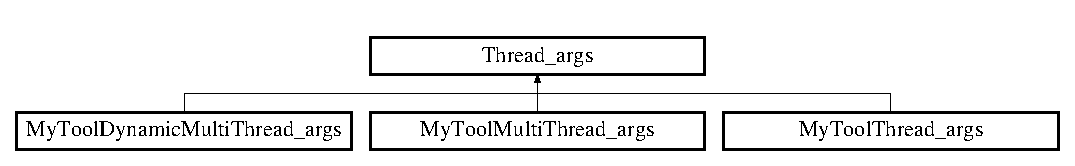
\includegraphics[height=10.000000cm]{structThread__args}
\end{center}
\end{figure}
\subsection*{Public Member Functions}
\begin{DoxyCompactItemize}
\item 
\hyperlink{structThread__args_a399b672e0f4f137fe52c141bd8c38eb1}{Thread\-\_\-args} ()
\item 
virtual \hyperlink{structThread__args_ad786e0c55b4e44bc04d9ba3b813bace1}{$\sim$\-Thread\-\_\-args} ()
\item 
\hyperlink{structThread__args_a399b672e0f4f137fe52c141bd8c38eb1}{Thread\-\_\-args} ()
\item 
virtual \hyperlink{structThread__args_ad786e0c55b4e44bc04d9ba3b813bace1}{$\sim$\-Thread\-\_\-args} ()
\item 
\hyperlink{structThread__args_a399b672e0f4f137fe52c141bd8c38eb1}{Thread\-\_\-args} ()
\item 
virtual \hyperlink{structThread__args_ad786e0c55b4e44bc04d9ba3b813bace1}{$\sim$\-Thread\-\_\-args} ()
\end{DoxyCompactItemize}
\subsection*{Public Attributes}
\begin{DoxyCompactItemize}
\item 
\hypertarget{structThread__args_a594f831be7ce66015a7606e023b24cf4}{std\-::string \hyperlink{structThread__args_a594f831be7ce66015a7606e023b24cf4}{Thread\-Name}}\label{structThread__args_a594f831be7ce66015a7606e023b24cf4}

\begin{DoxyCompactList}\small\item\em name of thread (deffined at creation) \end{DoxyCompactList}\item 
\hypertarget{structThread__args_a674c5df8bb54ea3f96befbef2dfb1a78}{void($\ast$ \hyperlink{structThread__args_a674c5df8bb54ea3f96befbef2dfb1a78}{func} )(\hyperlink{structThread__args}{Thread\-\_\-args} $\ast$)}\label{structThread__args_a674c5df8bb54ea3f96befbef2dfb1a78}

\begin{DoxyCompactList}\small\item\em function pointer to thread with args \end{DoxyCompactList}\item 
\hypertarget{structThread__args_a4f71beb11e75d05269fc63ca7c19a8a9}{pthread\-\_\-t \hyperlink{structThread__args_a4f71beb11e75d05269fc63ca7c19a8a9}{thread}}\label{structThread__args_a4f71beb11e75d05269fc63ca7c19a8a9}

\begin{DoxyCompactList}\small\item\em Simple constructor underlying thread that interface is built ontop of. \end{DoxyCompactList}\item 
\hypertarget{structThread__args_a9cb8f6b709c5687bf28531bf4d808c75}{bool \hyperlink{structThread__args_a9cb8f6b709c5687bf28531bf4d808c75}{running}}\label{structThread__args_a9cb8f6b709c5687bf28531bf4d808c75}

\begin{DoxyCompactList}\small\item\em Bool flag to tell the thread to run (if not set thread goes into wait cycle. \end{DoxyCompactList}\item 
\hypertarget{structThread__args_a298b8c85c8598ecc557e2090d90a73c3}{bool \hyperlink{structThread__args_a298b8c85c8598ecc557e2090d90a73c3}{kill}}\label{structThread__args_a298b8c85c8598ecc557e2090d90a73c3}

\begin{DoxyCompactList}\small\item\em Bool flay used to kill the thread. \end{DoxyCompactList}\end{DoxyCompactItemize}


\subsection{Constructor \& Destructor Documentation}
\hypertarget{structThread__args_a399b672e0f4f137fe52c141bd8c38eb1}{\index{Thread\-\_\-args@{Thread\-\_\-args}!Thread\-\_\-args@{Thread\-\_\-args}}
\index{Thread\-\_\-args@{Thread\-\_\-args}!Thread_args@{Thread\-\_\-args}}
\subsubsection[{Thread\-\_\-args}]{\setlength{\rightskip}{0pt plus 5cm}Thread\-\_\-args\-::\-Thread\-\_\-args (
\begin{DoxyParamCaption}
{}
\end{DoxyParamCaption}
)\hspace{0.3cm}{\ttfamily [inline]}}}\label{structThread__args_a399b672e0f4f137fe52c141bd8c38eb1}
$<$ Simple constructor \hypertarget{structThread__args_ad786e0c55b4e44bc04d9ba3b813bace1}{\index{Thread\-\_\-args@{Thread\-\_\-args}!$\sim$\-Thread\-\_\-args@{$\sim$\-Thread\-\_\-args}}
\index{$\sim$\-Thread\-\_\-args@{$\sim$\-Thread\-\_\-args}!Thread_args@{Thread\-\_\-args}}
\subsubsection[{$\sim$\-Thread\-\_\-args}]{\setlength{\rightskip}{0pt plus 5cm}virtual Thread\-\_\-args\-::$\sim$\-Thread\-\_\-args (
\begin{DoxyParamCaption}
{}
\end{DoxyParamCaption}
)\hspace{0.3cm}{\ttfamily [inline]}, {\ttfamily [virtual]}}}\label{structThread__args_ad786e0c55b4e44bc04d9ba3b813bace1}
$<$ virtual constructor \hypertarget{structThread__args_a399b672e0f4f137fe52c141bd8c38eb1}{\index{Thread\-\_\-args@{Thread\-\_\-args}!Thread\-\_\-args@{Thread\-\_\-args}}
\index{Thread\-\_\-args@{Thread\-\_\-args}!Thread_args@{Thread\-\_\-args}}
\subsubsection[{Thread\-\_\-args}]{\setlength{\rightskip}{0pt plus 5cm}Thread\-\_\-args\-::\-Thread\-\_\-args (
\begin{DoxyParamCaption}
{}
\end{DoxyParamCaption}
)\hspace{0.3cm}{\ttfamily [inline]}}}\label{structThread__args_a399b672e0f4f137fe52c141bd8c38eb1}
$<$ Simple constructor \hypertarget{structThread__args_ad786e0c55b4e44bc04d9ba3b813bace1}{\index{Thread\-\_\-args@{Thread\-\_\-args}!$\sim$\-Thread\-\_\-args@{$\sim$\-Thread\-\_\-args}}
\index{$\sim$\-Thread\-\_\-args@{$\sim$\-Thread\-\_\-args}!Thread_args@{Thread\-\_\-args}}
\subsubsection[{$\sim$\-Thread\-\_\-args}]{\setlength{\rightskip}{0pt plus 5cm}virtual Thread\-\_\-args\-::$\sim$\-Thread\-\_\-args (
\begin{DoxyParamCaption}
{}
\end{DoxyParamCaption}
)\hspace{0.3cm}{\ttfamily [inline]}, {\ttfamily [virtual]}}}\label{structThread__args_ad786e0c55b4e44bc04d9ba3b813bace1}
$<$ virtual constructor \hypertarget{structThread__args_a399b672e0f4f137fe52c141bd8c38eb1}{\index{Thread\-\_\-args@{Thread\-\_\-args}!Thread\-\_\-args@{Thread\-\_\-args}}
\index{Thread\-\_\-args@{Thread\-\_\-args}!Thread_args@{Thread\-\_\-args}}
\subsubsection[{Thread\-\_\-args}]{\setlength{\rightskip}{0pt plus 5cm}Thread\-\_\-args\-::\-Thread\-\_\-args (
\begin{DoxyParamCaption}
{}
\end{DoxyParamCaption}
)\hspace{0.3cm}{\ttfamily [inline]}}}\label{structThread__args_a399b672e0f4f137fe52c141bd8c38eb1}
$<$ Simple constructor \hypertarget{structThread__args_ad786e0c55b4e44bc04d9ba3b813bace1}{\index{Thread\-\_\-args@{Thread\-\_\-args}!$\sim$\-Thread\-\_\-args@{$\sim$\-Thread\-\_\-args}}
\index{$\sim$\-Thread\-\_\-args@{$\sim$\-Thread\-\_\-args}!Thread_args@{Thread\-\_\-args}}
\subsubsection[{$\sim$\-Thread\-\_\-args}]{\setlength{\rightskip}{0pt plus 5cm}virtual Thread\-\_\-args\-::$\sim$\-Thread\-\_\-args (
\begin{DoxyParamCaption}
{}
\end{DoxyParamCaption}
)\hspace{0.3cm}{\ttfamily [inline]}, {\ttfamily [virtual]}}}\label{structThread__args_ad786e0c55b4e44bc04d9ba3b813bace1}
$<$ virtual constructor 

The documentation for this struct was generated from the following files\-:\begin{DoxyCompactItemize}
\item 
Data\-Model/Utilities.\-h\item 
include/Utilities.\-h\item 
install/include/Utilities.\-h\end{DoxyCompactItemize}

\hypertarget{classTool}{\section{Tool Class Reference}
\label{classTool}\index{Tool@{Tool}}
}


{\ttfamily \#include $<$Tool.\-h$>$}

Inheritance diagram for Tool\-:\begin{figure}[H]
\begin{center}
\leavevmode
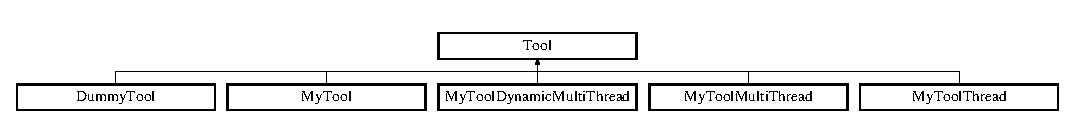
\includegraphics[height=11.000000cm]{classTool}
\end{center}
\end{figure}
\subsection*{Public Member Functions}
\begin{DoxyCompactItemize}
\item 
virtual bool \hyperlink{classTool_a4b04a99172dfe09dc97927d1feaff0ce}{Initialise} (std\-::string configfile, \hyperlink{classDataModel}{Data\-Model} \&data)=0
\begin{DoxyCompactList}\small\item\em virtual Initialise function that reads in the assigned config file and optain Data\-Moodel reference \end{DoxyCompactList}\item 
\hypertarget{classTool_a6a71469fa4efffd6fb71afbd4941e49d}{virtual bool \hyperlink{classTool_a6a71469fa4efffd6fb71afbd4941e49d}{Execute} ()=0}\label{classTool_a6a71469fa4efffd6fb71afbd4941e49d}

\begin{DoxyCompactList}\small\item\em Virtual Execute function. \end{DoxyCompactList}\item 
\hypertarget{classTool_a1f9a82fe5cc9afd63fc8eb3aaf5d80ca}{virtual bool \hyperlink{classTool_a1f9a82fe5cc9afd63fc8eb3aaf5d80ca}{Finalise} ()=0}\label{classTool_a1f9a82fe5cc9afd63fc8eb3aaf5d80ca}

\begin{DoxyCompactList}\small\item\em Virtual Finalise function. \end{DoxyCompactList}\item 
virtual bool \hyperlink{classTool_a4b04a99172dfe09dc97927d1feaff0ce}{Initialise} (std\-::string configfile, \hyperlink{classDataModel}{Data\-Model} \&data)=0
\begin{DoxyCompactList}\small\item\em virtual Initialise function that reads in the assigned config file and optain Data\-Moodel reference \end{DoxyCompactList}\item 
\hypertarget{classTool_a6a71469fa4efffd6fb71afbd4941e49d}{virtual bool \hyperlink{classTool_a6a71469fa4efffd6fb71afbd4941e49d}{Execute} ()=0}\label{classTool_a6a71469fa4efffd6fb71afbd4941e49d}

\begin{DoxyCompactList}\small\item\em Virtual Execute function. \end{DoxyCompactList}\item 
\hypertarget{classTool_a1f9a82fe5cc9afd63fc8eb3aaf5d80ca}{virtual bool \hyperlink{classTool_a1f9a82fe5cc9afd63fc8eb3aaf5d80ca}{Finalise} ()=0}\label{classTool_a1f9a82fe5cc9afd63fc8eb3aaf5d80ca}

\begin{DoxyCompactList}\small\item\em Virtual Finalise function. \end{DoxyCompactList}\end{DoxyCompactItemize}
\subsection*{Protected Member Functions}
\begin{DoxyCompactItemize}
\item 
\hyperlink{structMsgL}{Msg\-L} \hyperlink{classTool_aece350bc23e63656276b8338419dc54e}{M\-L} (int messagelevel)
\begin{DoxyCompactList}\small\item\em Function for setting logging level instream. \end{DoxyCompactList}\item 
\hypertarget{classTool_ae4da557812278419f6f8b8484df08115}{void \hyperlink{classTool_ae4da557812278419f6f8b8484df08115}{M\-L\-C} ()}\label{classTool_ae4da557812278419f6f8b8484df08115}

\begin{DoxyCompactList}\small\item\em Function for clearing logging level. \end{DoxyCompactList}\item 
\hypertarget{classTool_a46f7e599888302feefcf25e4f6cb4f9e}{{\footnotesize template$<$typename T $>$ }\\void {\bfseries Log} (T message, int messagelevel=1, int verbosity=1)}\label{classTool_a46f7e599888302feefcf25e4f6cb4f9e}

\item 
{\footnotesize template$<$typename T $>$ }\\void \hyperlink{classTool_ac65a2dfa2e3531fe8e05fe4112846fcf}{Log} (T message, int messagelevel)
\begin{DoxyCompactList}\small\item\em \hyperlink{classLogging}{Logging} fuction for printouts. \end{DoxyCompactList}\item 
\hyperlink{structMsgL}{Msg\-L} \hyperlink{classTool_aece350bc23e63656276b8338419dc54e}{M\-L} (int messagelevel)
\begin{DoxyCompactList}\small\item\em Function for setting logging level instream. \end{DoxyCompactList}\item 
\hypertarget{classTool_ae4da557812278419f6f8b8484df08115}{void \hyperlink{classTool_ae4da557812278419f6f8b8484df08115}{M\-L\-C} ()}\label{classTool_ae4da557812278419f6f8b8484df08115}

\begin{DoxyCompactList}\small\item\em Function for clearing logging level. \end{DoxyCompactList}\item 
\hypertarget{classTool_a46f7e599888302feefcf25e4f6cb4f9e}{{\footnotesize template$<$typename T $>$ }\\void {\bfseries Log} (T message, int messagelevel=1, int verbosity=1)}\label{classTool_a46f7e599888302feefcf25e4f6cb4f9e}

\item 
{\footnotesize template$<$typename T $>$ }\\void \hyperlink{classTool_ac65a2dfa2e3531fe8e05fe4112846fcf}{Log} (T message, int messagelevel)
\begin{DoxyCompactList}\small\item\em \hyperlink{classLogging}{Logging} fuction for printouts. \end{DoxyCompactList}\end{DoxyCompactItemize}
\subsection*{Protected Attributes}
\begin{DoxyCompactItemize}
\item 
\hyperlink{classStore}{Store} \hyperlink{classTool_a208aed50c1c50212d2927b372c38763f}{m\-\_\-variables}
\begin{DoxyCompactList}\small\item\em virtual destructor. \end{DoxyCompactList}\item 
\hypertarget{classTool_a0c166968759706b4cd07466693cf19d0}{\hyperlink{classDataModel}{Data\-Model} $\ast$ \hyperlink{classTool_a0c166968759706b4cd07466693cf19d0}{m\-\_\-data}}\label{classTool_a0c166968759706b4cd07466693cf19d0}

\begin{DoxyCompactList}\small\item\em Pointer to transiant \hyperlink{classDataModel}{Data\-Model} class. \end{DoxyCompactList}\item 
\hypertarget{classTool_ae769d2a46a51a2ab638b9d9fb1b78cb7}{\hyperlink{classLogging}{Logging} $\ast$ \hyperlink{classTool_ae769d2a46a51a2ab638b9d9fb1b78cb7}{m\-\_\-log}}\label{classTool_ae769d2a46a51a2ab638b9d9fb1b78cb7}

\begin{DoxyCompactList}\small\item\em Pointer to logging class. \end{DoxyCompactList}\item 
\hypertarget{classTool_a49dc4701c181ce95f8ca4699d82f34e5}{int \hyperlink{classTool_a49dc4701c181ce95f8ca4699d82f34e5}{m\-\_\-verbose}}\label{classTool_a49dc4701c181ce95f8ca4699d82f34e5}

\begin{DoxyCompactList}\small\item\em verbosity variable for direct logging level \end{DoxyCompactList}\end{DoxyCompactItemize}


\subsection{Detailed Description}
Abstract base class for Tools to inherit from. This allows a polymphic interface for the factor to use.

\begin{DoxyParagraph}{Author\-:}
B.\-Richards 
\end{DoxyParagraph}
\begin{DoxyParagraph}{Date\-:}
2019/05/28 10\-:44\-:00 
\end{DoxyParagraph}
Contact\-: \href{mailto:b.richards@qmul.ac.uk}{\tt b.\-richards@qmul.\-ac.\-uk} 

\subsection{Member Function Documentation}
\hypertarget{classTool_a4b04a99172dfe09dc97927d1feaff0ce}{\index{Tool@{Tool}!Initialise@{Initialise}}
\index{Initialise@{Initialise}!Tool@{Tool}}
\subsubsection[{Initialise}]{\setlength{\rightskip}{0pt plus 5cm}virtual bool Tool\-::\-Initialise (
\begin{DoxyParamCaption}
\item[{std\-::string}]{configfile, }
\item[{{\bf Data\-Model} \&}]{data}
\end{DoxyParamCaption}
)\hspace{0.3cm}{\ttfamily [pure virtual]}}}\label{classTool_a4b04a99172dfe09dc97927d1feaff0ce}


virtual Initialise function that reads in the assigned config file and optain Data\-Moodel reference 


\begin{DoxyParams}{Parameters}
{\em configfile} & Path and name of config file to read in. \\
\hline
{\em data} & Reference to \hyperlink{classDataModel}{Data\-Model}. \\
\hline
\end{DoxyParams}


Implemented in \hyperlink{classMyToolDynamicMultiThread_ac082408d85bc3e76214e55d4f62de0da}{My\-Tool\-Dynamic\-Multi\-Thread}, \hyperlink{classMyToolMultiThread_a19dc55079a7b2da02ad9addd565b8e80}{My\-Tool\-Multi\-Thread}, \hyperlink{classMyToolDynamicMultiThread_ac082408d85bc3e76214e55d4f62de0da}{My\-Tool\-Dynamic\-Multi\-Thread}, \hyperlink{classMyToolMultiThread_a19dc55079a7b2da02ad9addd565b8e80}{My\-Tool\-Multi\-Thread}, \hyperlink{classMyToolThread_adc7ab1ab74fc1564f07e52e63383d679}{My\-Tool\-Thread}, \hyperlink{classMyToolThread_adc7ab1ab74fc1564f07e52e63383d679}{My\-Tool\-Thread}, \hyperlink{classMyTool_a3bf60061195a18542c4cfb2916b9dad9}{My\-Tool}, \hyperlink{classMyTool_a3bf60061195a18542c4cfb2916b9dad9}{My\-Tool}, \hyperlink{classDummyTool_a0d9cd781681a06ee3cf0cd1e7bb770a8}{Dummy\-Tool}, and \hyperlink{classDummyTool_a0d9cd781681a06ee3cf0cd1e7bb770a8}{Dummy\-Tool}.

\hypertarget{classTool_a4b04a99172dfe09dc97927d1feaff0ce}{\index{Tool@{Tool}!Initialise@{Initialise}}
\index{Initialise@{Initialise}!Tool@{Tool}}
\subsubsection[{Initialise}]{\setlength{\rightskip}{0pt plus 5cm}virtual bool Tool\-::\-Initialise (
\begin{DoxyParamCaption}
\item[{std\-::string}]{configfile, }
\item[{{\bf Data\-Model} \&}]{data}
\end{DoxyParamCaption}
)\hspace{0.3cm}{\ttfamily [pure virtual]}}}\label{classTool_a4b04a99172dfe09dc97927d1feaff0ce}


virtual Initialise function that reads in the assigned config file and optain Data\-Moodel reference 


\begin{DoxyParams}{Parameters}
{\em configfile} & Path and name of config file to read in. \\
\hline
{\em data} & Reference to \hyperlink{classDataModel}{Data\-Model}. \\
\hline
\end{DoxyParams}


Implemented in \hyperlink{classMyToolDynamicMultiThread_ac082408d85bc3e76214e55d4f62de0da}{My\-Tool\-Dynamic\-Multi\-Thread}, \hyperlink{classMyToolMultiThread_a19dc55079a7b2da02ad9addd565b8e80}{My\-Tool\-Multi\-Thread}, \hyperlink{classMyToolDynamicMultiThread_ac082408d85bc3e76214e55d4f62de0da}{My\-Tool\-Dynamic\-Multi\-Thread}, \hyperlink{classMyToolMultiThread_a19dc55079a7b2da02ad9addd565b8e80}{My\-Tool\-Multi\-Thread}, \hyperlink{classMyToolThread_adc7ab1ab74fc1564f07e52e63383d679}{My\-Tool\-Thread}, \hyperlink{classMyToolThread_adc7ab1ab74fc1564f07e52e63383d679}{My\-Tool\-Thread}, \hyperlink{classMyTool_a3bf60061195a18542c4cfb2916b9dad9}{My\-Tool}, \hyperlink{classMyTool_a3bf60061195a18542c4cfb2916b9dad9}{My\-Tool}, \hyperlink{classDummyTool_a0d9cd781681a06ee3cf0cd1e7bb770a8}{Dummy\-Tool}, and \hyperlink{classDummyTool_a0d9cd781681a06ee3cf0cd1e7bb770a8}{Dummy\-Tool}.

\hypertarget{classTool_ac65a2dfa2e3531fe8e05fe4112846fcf}{\index{Tool@{Tool}!Log@{Log}}
\index{Log@{Log}!Tool@{Tool}}
\subsubsection[{Log}]{\setlength{\rightskip}{0pt plus 5cm}template$<$typename T $>$ void Tool\-::\-Log (
\begin{DoxyParamCaption}
\item[{T}]{message, }
\item[{int}]{messagelevel}
\end{DoxyParamCaption}
)\hspace{0.3cm}{\ttfamily [inline]}, {\ttfamily [protected]}}}\label{classTool_ac65a2dfa2e3531fe8e05fe4112846fcf}


\hyperlink{classLogging}{Logging} fuction for printouts. 


\begin{DoxyParams}{Parameters}
{\em message} & Templated message string. \\
\hline
{\em messagelevel} & The verbosity level at which to show the message. Checked against internal verbosity level \\
\hline
\end{DoxyParams}
\hypertarget{classTool_ac65a2dfa2e3531fe8e05fe4112846fcf}{\index{Tool@{Tool}!Log@{Log}}
\index{Log@{Log}!Tool@{Tool}}
\subsubsection[{Log}]{\setlength{\rightskip}{0pt plus 5cm}template$<$typename T $>$ void Tool\-::\-Log (
\begin{DoxyParamCaption}
\item[{T}]{message, }
\item[{int}]{messagelevel}
\end{DoxyParamCaption}
)\hspace{0.3cm}{\ttfamily [inline]}, {\ttfamily [protected]}}}\label{classTool_ac65a2dfa2e3531fe8e05fe4112846fcf}


\hyperlink{classLogging}{Logging} fuction for printouts. 


\begin{DoxyParams}{Parameters}
{\em message} & Templated message string. \\
\hline
{\em messagelevel} & The verbosity level at which to show the message. Checked against internal verbosity level \\
\hline
\end{DoxyParams}
\hypertarget{classTool_aece350bc23e63656276b8338419dc54e}{\index{Tool@{Tool}!M\-L@{M\-L}}
\index{M\-L@{M\-L}!Tool@{Tool}}
\subsubsection[{M\-L}]{\setlength{\rightskip}{0pt plus 5cm}{\bf Msg\-L} Tool\-::\-M\-L (
\begin{DoxyParamCaption}
\item[{int}]{messagelevel}
\end{DoxyParamCaption}
)\hspace{0.3cm}{\ttfamily [inline]}, {\ttfamily [protected]}}}\label{classTool_aece350bc23e63656276b8338419dc54e}


Function for setting logging level instream. 


\begin{DoxyParams}{Parameters}
{\em messagelevel} & the verboisty level at which to show the message. Checked against internal verbosity level. \\
\hline
\end{DoxyParams}
\hypertarget{classTool_aece350bc23e63656276b8338419dc54e}{\index{Tool@{Tool}!M\-L@{M\-L}}
\index{M\-L@{M\-L}!Tool@{Tool}}
\subsubsection[{M\-L}]{\setlength{\rightskip}{0pt plus 5cm}{\bf Msg\-L} Tool\-::\-M\-L (
\begin{DoxyParamCaption}
\item[{int}]{messagelevel}
\end{DoxyParamCaption}
)\hspace{0.3cm}{\ttfamily [inline]}, {\ttfamily [protected]}}}\label{classTool_aece350bc23e63656276b8338419dc54e}


Function for setting logging level instream. 


\begin{DoxyParams}{Parameters}
{\em messagelevel} & the verboisty level at which to show the message. Checked against internal verbosity level. \\
\hline
\end{DoxyParams}


\subsection{Member Data Documentation}
\hypertarget{classTool_a208aed50c1c50212d2927b372c38763f}{\index{Tool@{Tool}!m\-\_\-variables@{m\-\_\-variables}}
\index{m\-\_\-variables@{m\-\_\-variables}!Tool@{Tool}}
\subsubsection[{m\-\_\-variables}]{\setlength{\rightskip}{0pt plus 5cm}{\bf Store} Tool\-::m\-\_\-variables\hspace{0.3cm}{\ttfamily [protected]}}}\label{classTool_a208aed50c1c50212d2927b372c38763f}


virtual destructor. 

\hyperlink{classStore}{Store} used to store configuration varaibles 

The documentation for this class was generated from the following files\-:\begin{DoxyCompactItemize}
\item 
include/Tool.\-h\item 
src/\-Tool/Tool.\-h\end{DoxyCompactItemize}

\hypertarget{classToolChain}{\section{Tool\-Chain Class Reference}
\label{classToolChain}\index{Tool\-Chain@{Tool\-Chain}}
}


{\ttfamily \#include $<$Tool\-Chain.\-h$>$}

\subsection*{Public Member Functions}
\begin{DoxyCompactItemize}
\item 
\hyperlink{classToolChain_a133e224899a743ee4a679396f8569bf9}{Tool\-Chain} (std\-::string configfile, int argc=0, char $\ast$argv\mbox{[}$\,$\mbox{]}=0)
\begin{DoxyCompactList}\small\item\em Constructor that obtains all of the configuration varaibles from an input file. \end{DoxyCompactList}\item 
\hyperlink{classToolChain_adefb544d73c43c2621f3ccb14ad93dc7}{Tool\-Chain} (int verbose=1, int errorlevel=0, bool log\-\_\-interactive=true, bool log\-\_\-local=false, std\-::string log\-\_\-local\-\_\-path=\char`\"{}./log\char`\"{}, bool log\-\_\-split\-\_\-files=false, \hyperlink{classDataModel}{Data\-Model} $\ast$in\-\_\-data\-\_\-model=0)
\item 
bool \hyperlink{classToolChain_ae6859092e14be1f9538c50d7c838fe8e}{Add} (std\-::string name, \hyperlink{classTool}{Tool} $\ast$tool, std\-::string configfile=\char`\"{}\char`\"{})
\begin{DoxyCompactList}\small\item\em Add a \hyperlink{classTool}{Tool} to the \hyperlink{classToolChain}{Tool\-Chain}. \end{DoxyCompactList}\item 
\hypertarget{classToolChain_a341f343926341b82a29c586a7b9683af}{int \hyperlink{classToolChain_a341f343926341b82a29c586a7b9683af}{Initialise} ()}\label{classToolChain_a341f343926341b82a29c586a7b9683af}

\begin{DoxyCompactList}\small\item\em Initialise all Tools in the \hyperlink{classToolChain}{Tool\-Chain} sequentially. \end{DoxyCompactList}\item 
int \hyperlink{classToolChain_a303e299293fd4d3a5e91865e04898e52}{Execute} (int repeates=1)
\begin{DoxyCompactList}\small\item\em Execute all Tools in the \hyperlink{classToolChain}{Tool\-Chain} sequentially. \end{DoxyCompactList}\item 
\hypertarget{classToolChain_a3828756135773fb9ca4b361a47296dd9}{int \hyperlink{classToolChain_a3828756135773fb9ca4b361a47296dd9}{Finalise} ()}\label{classToolChain_a3828756135773fb9ca4b361a47296dd9}

\begin{DoxyCompactList}\small\item\em Finalise all Tools in the Tool\-Cahin sequentially. \end{DoxyCompactList}\item 
\hypertarget{classToolChain_a9bb47b83b6b85c3b0fab75af0cda19bf}{void \hyperlink{classToolChain_a9bb47b83b6b85c3b0fab75af0cda19bf}{Interactive} ()}\label{classToolChain_a9bb47b83b6b85c3b0fab75af0cda19bf}

\begin{DoxyCompactList}\small\item\em Start interactive thread to accept commands and run \hyperlink{classToolChain}{Tool\-Chain} in interactive mode. \end{DoxyCompactList}\item 
\hypertarget{classToolChain_ac1b120b81163d9e00ee778fbc40ddb23}{bool {\bfseries Load\-Tools} (std\-::string filename)}\label{classToolChain_ac1b120b81163d9e00ee778fbc40ddb23}

\end{DoxyCompactItemize}
\subsection*{Public Attributes}
\begin{DoxyCompactItemize}
\item 
\hypertarget{classToolChain_a29d8574ddfd60c6fee03891c1eb6848c}{\hyperlink{classDataModel}{Data\-Model} $\ast$ \hyperlink{classToolChain_a29d8574ddfd60c6fee03891c1eb6848c}{m\-\_\-data}}\label{classToolChain_a29d8574ddfd60c6fee03891c1eb6848c}

\begin{DoxyCompactList}\small\item\em Direct access to transient data model class of the Tools in the \hyperlink{classToolChain}{Tool\-Chain}. This allows direct initialisation and copying of variables. \end{DoxyCompactList}\end{DoxyCompactItemize}
\subsection*{Protected Member Functions}
\begin{DoxyCompactItemize}
\item 
\hypertarget{classToolChain_ab705c173cb72d1d35865f7435bcb9f0b}{virtual void {\bfseries Init} ()}\label{classToolChain_ab705c173cb72d1d35865f7435bcb9f0b}

\item 
\hypertarget{classToolChain_ac1cc0e9d9f6b2d23adb9eab2d7a58119}{void {\bfseries Inline} ()}\label{classToolChain_ac1cc0e9d9f6b2d23adb9eab2d7a58119}

\item 
\hypertarget{classToolChain_a6ce65465365bf2b6da10b5d28028afcb}{std\-::string {\bfseries Execute\-Command} (std\-::string connand)}\label{classToolChain_a6ce65465365bf2b6da10b5d28028afcb}

\end{DoxyCompactItemize}
\subsection*{Static Protected Member Functions}
\begin{DoxyCompactItemize}
\item 
\hypertarget{classToolChain_a7f6fcdce202336463b71aa5167758bd2}{static void $\ast$ {\bfseries Interactive\-Thread} (void $\ast$arg)}\label{classToolChain_a7f6fcdce202336463b71aa5167758bd2}

\end{DoxyCompactItemize}
\subsection*{Protected Attributes}
\begin{DoxyCompactItemize}
\item 
\hypertarget{classToolChain_a5327190043dfcdc67affc35ddb836c68}{std\-::vector$<$ \hyperlink{classTool}{Tool} $\ast$ $>$ {\bfseries m\-\_\-tools}}\label{classToolChain_a5327190043dfcdc67affc35ddb836c68}

\item 
\hypertarget{classToolChain_ab88ccb68da6feb135c032f1356a4889f}{std\-::vector$<$ std\-::string $>$ {\bfseries m\-\_\-toolnames}}\label{classToolChain_ab88ccb68da6feb135c032f1356a4889f}

\item 
\hypertarget{classToolChain_a74cb5832ff5a41714a4da2448b87cee6}{std\-::vector$<$ std\-::string $>$ {\bfseries m\-\_\-configfiles}}\label{classToolChain_a74cb5832ff5a41714a4da2448b87cee6}

\item 
\hypertarget{classToolChain_a3e157c7148cbdb9eccd43fce185297f5}{int {\bfseries m\-\_\-verbose}}\label{classToolChain_a3e157c7148cbdb9eccd43fce185297f5}

\item 
\hypertarget{classToolChain_a26843fabb52f0fba5f91be3da7564e4e}{int {\bfseries m\-\_\-errorlevel}}\label{classToolChain_a26843fabb52f0fba5f91be3da7564e4e}

\item 
\hypertarget{classToolChain_a0c1470a33c6f3f2749230ed4b2165c5b}{bool {\bfseries m\-\_\-log\-\_\-interactive}}\label{classToolChain_a0c1470a33c6f3f2749230ed4b2165c5b}

\item 
\hypertarget{classToolChain_a2076a51d02b80034f523b332ddd452c3}{bool {\bfseries m\-\_\-log\-\_\-local}}\label{classToolChain_a2076a51d02b80034f523b332ddd452c3}

\item 
\hypertarget{classToolChain_a0aa84e0beb152870363f4c7a23466c15}{bool {\bfseries m\-\_\-log\-\_\-split\-\_\-files}}\label{classToolChain_a0aa84e0beb152870363f4c7a23466c15}

\item 
\hypertarget{classToolChain_a030b1214102cfb02242e2247248f6087}{std\-::string {\bfseries m\-\_\-log\-\_\-local\-\_\-path}}\label{classToolChain_a030b1214102cfb02242e2247248f6087}

\item 
\hypertarget{classToolChain_a1ed4e371b26c220f0018ad54dc2260fd}{bool {\bfseries m\-\_\-interactive}}\label{classToolChain_a1ed4e371b26c220f0018ad54dc2260fd}

\item 
\hypertarget{classToolChain_a9fc8417d6708585de3d4b96a49709a3c}{int {\bfseries m\-\_\-inline}}\label{classToolChain_a9fc8417d6708585de3d4b96a49709a3c}

\item 
\hypertarget{classToolChain_ace512f7eff07742d545cd9c15cf2b3c0}{bool {\bfseries m\-\_\-recover}}\label{classToolChain_ace512f7eff07742d545cd9c15cf2b3c0}

\item 
\hypertarget{classToolChain_a408cf3ba3c040374fa00ac4b789712cd}{bool {\bfseries exeloop}}\label{classToolChain_a408cf3ba3c040374fa00ac4b789712cd}

\item 
\hypertarget{classToolChain_a97ae31bc6524d2dcec465eadbde52bb1}{unsigned long {\bfseries execounter}}\label{classToolChain_a97ae31bc6524d2dcec465eadbde52bb1}

\item 
\hypertarget{classToolChain_a183dede9901ee79ed7c52b41f7d4b3b4}{bool {\bfseries Initialised}}\label{classToolChain_a183dede9901ee79ed7c52b41f7d4b3b4}

\item 
\hypertarget{classToolChain_ac52f9abf9a9df10846ad77ecd48b3065}{bool {\bfseries Finalised}}\label{classToolChain_ac52f9abf9a9df10846ad77ecd48b3065}

\item 
\hypertarget{classToolChain_a047c9aa0130323fd4fa7a0065e18e1f2}{bool {\bfseries paused}}\label{classToolChain_a047c9aa0130323fd4fa7a0065e18e1f2}

\item 
\hypertarget{classToolChain_a6454194aa230cf3fed8858fbfb20f8c6}{\hyperlink{classLogging}{Logging} $\ast$ {\bfseries m\-\_\-log}}\label{classToolChain_a6454194aa230cf3fed8858fbfb20f8c6}

\item 
\hypertarget{classToolChain_a057de33170307a943960230206bb69b2}{pthread\-\_\-t {\bfseries thread} \mbox{[}1\mbox{]}}\label{classToolChain_a057de33170307a943960230206bb69b2}

\item 
\hypertarget{classToolChain_a621ee785109fba1cb9def121a2ada524}{bool {\bfseries msgflag}}\label{classToolChain_a621ee785109fba1cb9def121a2ada524}

\end{DoxyCompactItemize}


\subsection{Detailed Description}
This class holds a dynamic list of Tools which can be Initialised, Executed and Finalised to perform program operation. Large number of options in terms of run modes and setting can be assigned.

\begin{DoxyParagraph}{Author\-:}
B.\-Richards 
\end{DoxyParagraph}
\begin{DoxyParagraph}{Date\-:}
2019/05/28 10\-:44\-:00 
\end{DoxyParagraph}


\subsection{Constructor \& Destructor Documentation}
\hypertarget{classToolChain_a133e224899a743ee4a679396f8569bf9}{\index{Tool\-Chain@{Tool\-Chain}!Tool\-Chain@{Tool\-Chain}}
\index{Tool\-Chain@{Tool\-Chain}!ToolChain@{Tool\-Chain}}
\subsubsection[{Tool\-Chain}]{\setlength{\rightskip}{0pt plus 5cm}Tool\-Chain\-::\-Tool\-Chain (
\begin{DoxyParamCaption}
\item[{std\-::string}]{configfile, }
\item[{int}]{argc = {\ttfamily 0}, }
\item[{char $\ast$}]{argv\mbox{[}$\,$\mbox{]} = {\ttfamily 0}}
\end{DoxyParamCaption}
)}}\label{classToolChain_a133e224899a743ee4a679396f8569bf9}


Constructor that obtains all of the configuration varaibles from an input file. 


\begin{DoxyParams}{Parameters}
{\em configfile} & The path and name of the config file to read configuration values from. \\
\hline
\end{DoxyParams}
\hypertarget{classToolChain_adefb544d73c43c2621f3ccb14ad93dc7}{\index{Tool\-Chain@{Tool\-Chain}!Tool\-Chain@{Tool\-Chain}}
\index{Tool\-Chain@{Tool\-Chain}!ToolChain@{Tool\-Chain}}
\subsubsection[{Tool\-Chain}]{\setlength{\rightskip}{0pt plus 5cm}Tool\-Chain\-::\-Tool\-Chain (
\begin{DoxyParamCaption}
\item[{int}]{verbose = {\ttfamily 1}, }
\item[{int}]{errorlevel = {\ttfamily 0}, }
\item[{bool}]{log\-\_\-interactive = {\ttfamily true}, }
\item[{bool}]{log\-\_\-local = {\ttfamily false}, }
\item[{std\-::string}]{log\-\_\-local\-\_\-path = {\ttfamily \char`\"{}./log\char`\"{}}, }
\item[{bool}]{log\-\_\-split\-\_\-files = {\ttfamily false}, }
\item[{{\bf Data\-Model} $\ast$}]{in\-\_\-data\-\_\-model = {\ttfamily 0}}
\end{DoxyParamCaption}
)}}\label{classToolChain_adefb544d73c43c2621f3ccb14ad93dc7}
\begin{DoxyVerb} Constructor with explicit configuration variables passed as arguments.
 @param verbose The verbosity level of the ToolChain. The higher the number the more explicit the print outs. 0 = silent apart from errors.
 @param errorlevel The behavior that occurs when the ToolChain encounters an error. 0 = do not exit for both handeled and unhandeled errors, 1 = exit on unhandeled errors only, 2 = exit on handeled and unhandeled errors.
 @param log_interactive sets the logging class to use standard output and error to screen
 @param log_local sets the logging class to redirect standard output and error to disk
\end{DoxyVerb}
 logmode Where log printouts should be forwarded too. \char`\"{}\-Interactive\char`\"{} = cout, \char`\"{}\-Remote\char`\"{} = send to a remote logging system, \char`\"{}local\char`\"{} = ouput logs to a file. 
\begin{DoxyParams}{Parameters}
{\em log\-\_\-local\-\_\-path} & The file path and name of where to store logs if in Local logging mode. \\
\hline
{\em log\-\_\-split\-\_\-files} & when loggign to local file whether to split standard output and standard error into differnt files \\
\hline
{\em in\-\_\-data\-\_\-model} & option to specify an external data modle for use in \hyperlink{classToolChain}{Tool\-Chain}. \\
\hline
\end{DoxyParams}


\subsection{Member Function Documentation}
\hypertarget{classToolChain_ae6859092e14be1f9538c50d7c838fe8e}{\index{Tool\-Chain@{Tool\-Chain}!Add@{Add}}
\index{Add@{Add}!ToolChain@{Tool\-Chain}}
\subsubsection[{Add}]{\setlength{\rightskip}{0pt plus 5cm}bool Tool\-Chain\-::\-Add (
\begin{DoxyParamCaption}
\item[{std\-::string}]{name, }
\item[{{\bf Tool} $\ast$}]{tool, }
\item[{std\-::string}]{configfile = {\ttfamily \char`\"{}\char`\"{}}}
\end{DoxyParamCaption}
)}}\label{classToolChain_ae6859092e14be1f9538c50d7c838fe8e}


Add a \hyperlink{classTool}{Tool} to the \hyperlink{classToolChain}{Tool\-Chain}. 


\begin{DoxyParams}{Parameters}
{\em name} & The name used in logs when reffering to the \hyperlink{classTool}{Tool}. \\
\hline
{\em tool} & A pointer to the tool to be added to the \hyperlink{classToolChain}{Tool\-Chain}. \\
\hline
{\em configfile} & The configuration file path and name to be passed to the \hyperlink{classTool}{Tool}. \\
\hline
\end{DoxyParams}
\hypertarget{classToolChain_a303e299293fd4d3a5e91865e04898e52}{\index{Tool\-Chain@{Tool\-Chain}!Execute@{Execute}}
\index{Execute@{Execute}!ToolChain@{Tool\-Chain}}
\subsubsection[{Execute}]{\setlength{\rightskip}{0pt plus 5cm}int Tool\-Chain\-::\-Execute (
\begin{DoxyParamCaption}
\item[{int}]{repeates = {\ttfamily 1}}
\end{DoxyParamCaption}
)}}\label{classToolChain_a303e299293fd4d3a5e91865e04898e52}


Execute all Tools in the \hyperlink{classToolChain}{Tool\-Chain} sequentially. 


\begin{DoxyParams}{Parameters}
{\em repeates} & How many times to run sequential Execute loop. \\
\hline
\end{DoxyParams}


The documentation for this class was generated from the following files\-:\begin{DoxyCompactItemize}
\item 
src/\-Tool\-Chain/Tool\-Chain.\-h\item 
src/\-Tool\-Chain/Tool\-Chain.\-cpp\end{DoxyCompactItemize}

\hypertarget{structToolChainargs}{\section{Tool\-Chainargs Struct Reference}
\label{structToolChainargs}\index{Tool\-Chainargs@{Tool\-Chainargs}}
}


{\ttfamily \#include $<$Tool\-Chain.\-h$>$}

\subsection*{Public Attributes}
\begin{DoxyCompactItemize}
\item 
\hypertarget{structToolChainargs_a3551269b039d543b844a2d0d924ce96b}{bool $\ast$ \hyperlink{structToolChainargs_a3551269b039d543b844a2d0d924ce96b}{msgflag}}\label{structToolChainargs_a3551269b039d543b844a2d0d924ce96b}

\begin{DoxyCompactList}\small\item\em Message flag used to indiacte if a new interactive command has been submitted to the interactive thread and needs execution on the main thread. \end{DoxyCompactList}\item 
\hypertarget{structToolChainargs_a9d4c78b8b89eba4b7e8af9e6278c1bfd}{std\-::string {\bfseries command}}\label{structToolChainargs_a9d4c78b8b89eba4b7e8af9e6278c1bfd}

\end{DoxyCompactItemize}


\subsection{Detailed Description}
Simple struct to pass thread initalisation variables to Interactive \hyperlink{classToolChain}{Tool\-Chain} thread

\begin{DoxyParagraph}{Author\-:}
B.\-Richards 
\end{DoxyParagraph}
\begin{DoxyParagraph}{Date\-:}
2019/05/28 10\-:44\-:00 
\end{DoxyParagraph}


The documentation for this struct was generated from the following file\-:\begin{DoxyCompactItemize}
\item 
src/\-Tool\-Chain/Tool\-Chain.\-h\end{DoxyCompactItemize}

%--- End generated contents ---

% Index
\newpage
\phantomsection
\addcontentsline{toc}{part}{Index}
\printindex

\end{document}
